\chapter{Úvod}

V~dnešnej dobe sa bežný človek stretáva s~potrebou autentifikácie každý deň. Či už ide o~súkromné, pracovné alebo akademické účely. Na toto slúžia autentifikačné systémy rôznych foriem, úrovní bezpečnosti a princípov. Čoraz bežnejšie sú autentifikačné systémy založené na biometrických vlastnostiach. Ako býva zvykom, so vzostupom určitej technológie sa zároveň začnú objavovať aj spôsoby na jej skompromitovanie. Biometrické vlastnosti, na rozdiel od povedzme hesla alebo bankovej karty sa nedajú obnoviť, pretože sú pre každého človeka jedinečné a nemenné. Preto je nutné veľmi dôkladne dbať o~ich bezpečné uloženie a ochranu.

V~posledných rokoch taktiež pozorujeme vzostup technológie blockchain. Vďaka svojim vlastnostiam ako sú dôveryhodnosť, auditovateľnosť a nemennosť bola pôvodne zamýšľaná najmä ako prostriedok pre realizáciu kryptomien, no s~jej postupným rozšírením do povedomia verejnosti sa rozrástli aj možnosti jej využitia. S~príchodom blockchainu Ethereum boli spopularizované aj smart kontrakty, ktoré predstavovali kód spustiteľný v~bezpečnom prostredí siete blockchainu.

Hľadanie nových spôsobov ako zvýšiť bezpečnosť a dôveryhodnosť autentifikačných systémov viedlo ku zváženiu využitia technológie blockchain. V~tejto práci budú popísané princípy autentifikačných systémov súčasnosti, ako aj technológie blockchain.

\section{Cieľ práce}
Hlavným cieľom je navrhnúť biometrický autentifikačný systém schopný detekcie porušenia integrity úložiska biometrických šablón. Systém by mal využívať decentralizovaný prístup ku autentifikácii a byť implementovaný za využitia technológie blockchain. Navrhnutý systém bude následne otestovaný vzhľadom na funkčnosť a zhodnotený s~dôraznom na bezpečnosť.


\chapter{Autentifikačné systémy}
Pod týmto pojmom sa rozumie systém, ktorý vie potvrdiť identitu užívateľa. Spôsob autentifikácie môže mať viacero foriem, záleží od užívateľom poskytnutých informácií. Najčastejšou, najtradičnejšou formou je autentifikácia pomocou poskytnutia vopred dohodnutej informácie, najčastejšie má formu hesla \cite{authentication_systems1}.

\section{Vlastnosti}
Každý autentifikačný systém musí spĺňať určité vlastnosti, týkajúce sa najmä jeho bezpečnosti. Sú nimi integrita, dostupnosť a dôvernosť. Integrita reprezentuje schopnosť správne identifikovať jednotlivých overených užívateľov a spojiť ich so úkonmi, ktoré v~rámci systému vykonali. Zároveň zaručuje schopnosť systému znemožniť prístup neoprávneným užívateľom. Dôvernosťou sa rozumie jednak odolnosť voči získaniu autentifikačných prostriedkov pre vstup ale aj ochrana proti zneužitiu osobných údajov používateľa uložených v~systéme. Poslednou požiadavkou je dostupnosť systému pre overených používateľov, čiže odolnosť voči útokom typu odopretia služby.

Podľa spôsobu poznáme tri hlavné prístupy ku autentifikácii. Ich výber závisí na potrebách, zdrojoch a prioritách konkrétneho prípadu použitia \cite{authentication_systems2}.

\paragraph{Založené na znalosti (knowledge based)}
Pri tomto prístupe sa používateľ autentifikuje preukázaním znalosti určitej informácie. Tá má najčastejšie podobu dôverného hesla. Tento spôsob je zraniteľný voči viacerým metódam útokov založených na pokuse o~uhádnutie hesla, odpozorovaní hesla alebo zachytení komunikácie.

Metóda pokusu o~uhádnutie hesla spočíva v~útoku hrubou silou, kedy sa útočník snaží uhádnuť heslo vyskúšaním všetkých možných kombinácií. Tento typ útoku sa v~praxi ukázal ako časovo náročný, nakoľko s~dĺžkou hesla násobne stúpa aj čas potrebný na jeho uhádnutie. Toto viedlo ku modifikácii tejto metódy do podoby slovníkového útoku. Nutnosť čoraz väčšej dĺžky hesla však zvyšuje tendenciu užívateľov si heslo niekam napísať alebo znížiť jeho zložitosť. Práve znížením zložitosti sa stáva zraniteľné  voči slovníkovému útoku, ktorý namiesto skúšania všetkých možností vyskúša iba niekoľko najpravdepodobnejších slov.

Odpozorovanie užívateľa pri zadávaní hesla môže nastať ako fyzicky, užívateľ je nahraný videokamerou, prípadne pozorovaný pri zadávaní hesla, napríklad kamerou dodatočne umiestnenou na bankomat, ale aj cez softvér, ktorý zachytáva vstup z~klávesnice.

Odchytávanie a následný zásah do komunikácie medzi dvoma stranami má viacero foriem. Jenou z~nich je situácia man in the middle, ktorá spočíva vo vydávaní sa za obidve strany a následnom upravovaní vymieňaných správ podľa potreby. Jednoduchšou variantou, je replay útok, teda zachytenie dôkazu identity za úmyslom jeho neskoršieho použitia. Phishing je metóda zameraná na užívateľa, útočník sa pri nej vytvorí falošnú verziu autentifikačnej brány a následne sa pokúsi od užívateľa získať autentifikačnú informáciu na základe jeho nepozornosti.

\paragraph{Založené na vlastníctve (token based)}
Užívateľ sa autentifikuje preukázaním vlastníctva určitého autentifikačného tokenu. Tie môžu mať podobu čipovej karty ako je tomu pri bankových a prístupových kartách a dokladoch. Podstata tohto prístupu so sebou však nesie obmedzenie v~podobe potreby čítacieho zariadenia, ktoré je schopné potvrdiť autenticitu tokenu. Slabinou tohto prístupu je hrozba odcudzenia alebo neoprávneného kopírovania samotného tokenu. Z~tohto dôvodu sa v~kritických prípadoch používa autentifikačný token v~kombinácii s~ďalším spôsobom autentifikácie, najmä jednorazovým heslom.

\paragraph{Založené na biometrii}
Tento spôsob využíva unikátne nemenné biometrické vlastnosti ako dôkaz identity. Tie môžeme nájsť v~podobe fyzických čŕt a behaviorálnej charakteristiky jednotlivca. Fyzické črty sú napríklad odtlačok prsta a dlane, tvár, sietnica alebo dúhovka. Medzi behaviorálne charakteristiky patrí charakteristika písma, gestikulácia a hlas.

\section{Biometrické autentifikačné systémy}
Berme do úvahy systém, ktorý používa odtlačok prsta na autentifikáciu osoby. Ďalej budú popísané jeho vlastnosti a princípy.

\subsection{Princíp fungovania}
Samotný systém sa skladá z~viacerých komponentov, ktoré spolupracujú pri autentifikácií užívateľa \cite{biometric_systems_principle}.

\begin{itemize}
\item{Snímanie – realizované hardvérovým snímačom slúžiacim na získanie biometrických čŕt osoby. V~prípade autentifikačného systému založeného na odtlačkoch prsta je jeho úlohou vyhotoviť digitálnu snímku tvarov a záhybov nachádzajúcich sa na končeku prsta. Taktiež predstavuje hlavné rozhranie medzi používateľmi a systémom. Presnosť snímača je dôležitým parametrom nakoľko od nej závisí kvalita a použiteľnosť vyprodukovaných dát. 
}

\item{Predspracovanie – v~tomto kroku sa dáta poskytnuté snímačom vyčistia aplikovaním algoritmu na to určeného. Následne sa zhodnotí ich kvalita a miera použiteľnosti a v~prípade nekvalitnej vzorky je potrebné opakovať vyhotovenie digitálnej snímky.
}

\item{Extrakcia šablóny – táto časť má za úlohu spracovanie dát z~poskytnutých biometrických čŕt, ktoré budú slúžiť ako vstup pre overenie identity. Dáta extrahované z~biometrických čŕt sa všeobecne nazývajú biometrická šablóna.
}

\item{Databáza šablón – miesto kam sa ukladajú biometrické šablóny užívateľov evidovaných systémom. Databáza následne počas pokusu o~autentifikáciu poskytuje referenčné šablóny určené na porovnanie.
}

\item{Porovnanie – pri pokuse o~autentifikáciu sa z~databázy vyžiada referenčná šablón, ktorá sa porovná s~extrahovanou šablónou. Miera zhody extrahovaných dát s~referenčnou šablónou určí úspešnosť pokusu o~autentifikáciu. Úspešná autentifikácia nemusí nutne mať 100\% zhodu, nakoľko tá závisí od kvality vstupných dát.
}

\end{itemize}

\subsection{Možné útoky}
Ako každý systém, aj tento typ je zraniteľný voči niekoľkým typom útokov \ref{pic_auth_attacks}. Jednotlivé útoky sa líšia v~tom, na ktorú časť systému sú sústreďované \cite{biometric_authentication_threads1}.

\begin{figure}[hbt]
	\centering
	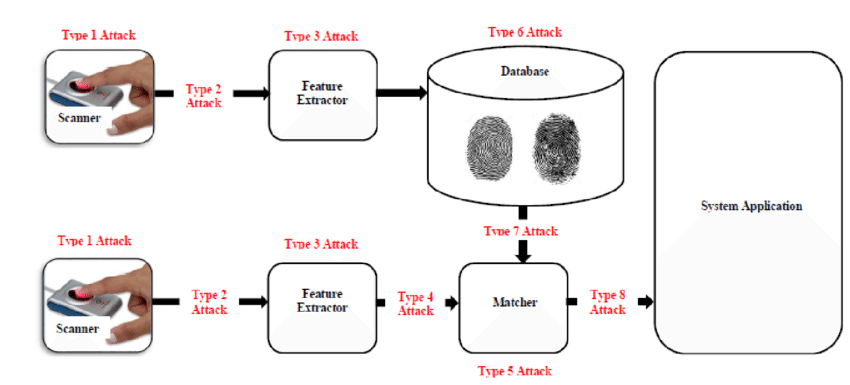
\includegraphics[width=\textwidth]{obrazky-figures/biometri-system-attacks.png}
	\caption{Vizualizácia možných útokov na biometrický systém \cite{biometric_authentication_threads1}.}
	\label{pic_auth_attacks}
\end{figure}

\begin{itemize}

\item{Útok na snímač (útok typu 1) – útočník môže vyrobiť fyzickú napodobeninu biometrických čŕt, v~tomto prípade umelý prst alebo môže vložiť umelo vytvorenú snímku odtlačku prsta medzi senzor snímača a jeho zvyšnú časť.
}

\item{Útok na komunikačný kanál medzi snímačom a extraktorom šablóny (útok typu 2) – po zosnímaní sú biometrické črty zaslané na ďalšie spracovanie do extraktora šablóny. Útok spočíva v~zachytení prenosu v~komunikačnom kanáli a nahradení originálnych dát vlastnými podľa potreby. Sem spadá taktiež útok typu replay, kedy útočník odpočúvaním komunikačného kanála odchytí pravé dáta užívateľa, ktoré neskôr použije na neoprávnený prístup do systému.
}

\item{Útok na extraktor rýs (útok typu 3) – útočník nahraní extraktor vlastným programom, ktorý vie jednak zhromažďovať zosnímané biometrické črty od užívateľov a taktiež vkladať do systému vlastné, podvrhnuté dáta

}

\item{Útok na komunikačný kanál medzi medzi extraktorom šablón a modulom porovnania (útok typu 4) – útočník sa pokúsi odchytiť extrahovanú šablónu a následne ju neskôr použije ako podvrhnutý vstup pre modul porovnania za účelom získania neoprávneného prístupu do systému (útok replay)
}

\item{Útok na modul porovnania (útok typu 5) – modul je nahradený podvrhnutým programom, ktorý aj pre neoprávneného užívateľa produkuje vysokú zhodu, ktorú následne signalizuje ďalej do systému. Pri tomto typu útoku nie je potrebné prehratie získaných údajov, jedná sa o~kompletné obídenie biometrického zabezpečenia systému.
}

\item{Útok na databázu biometrických šablón (útok typu 6) – prípad, kedy sa útočník skompromituje databázu pridaním, úpravou alebo vymazaním uložených biometrických šablón. Docieli toho využitím nedostatkov v~zabezpečení databázového softvéru alebo určitým spôsobom získa prístup ku správcovskému účtu.
}

\item{Útok na komunikačný kanál medzi modulom porovnania a databázou šablón (útok typu 7) – opäť ide o~odpočúvanie za účelom získania dát a ich neskoršieho použitia (replay útok)
}

\item{Útok na komunikačný kanál medzi modulom porovnania a databázou (útok typu 8) – útočník zamení dáta predávané medzi týmito časťami systému buď za svoje vlastné upravené podľa potreby alebo za pravé, skôr zachytené dáta
}
\end{itemize}


\chapter{Technológia Blockchain}
Jedná sa o~nemennú distribuovanú „účtovnú knihu“, ktorej obsah je viditeľný každému, kto sa na blockchaine podieľa. Slovo blockchain samé o~sebe naznačuje, že ide o~istý reťazec blokov, do ktorého sa neustále dynamicky pridávajú nové bloky obsahujúce dáta, ktoré majú byť pridané do blockchainu. Zmeny stavu blockchainu sa nazývajú transakcie. Ich vykonávanie prebieha distribuovane a decentralizovane, prostredníctvom podieľajúcich sa výpočtových uzlov v~sieti. Bezpečnosť a integrita dát v~blockchaine je zaistená pomocou konsenzus protokolov a asymetrickej kryptografie \cite{blockchain_architecture2}.

\section{História}
Prvá zmienka o~technológii podobnej blockchainu pochádza z~roku 1991, kedy S. Hauber a W. Scott popísali koncept kryptograficky zabezpečenej nadväzujúcej série blokov. Blockchain ako ho poznáme pochádza z~roku 2008, kedy vývojár alebo skupina vývojárov (identita do dnes nie je známa) pod pseudonymom Satoshi Nakamoto publikovala koncept elektronického peňažného systému s~názvom Bitcoin. Tento systém následne v~roku 2009 implementovali a nasadili, čím vznikla prvá kryptomena nesúca rovnomenný názov: Bitcoin \cite{blockchain_history1}.

Blockchain bol vo svojom pôvodnom koncepte určený exkluzívne ako prostriedok pre realizáciu kryptomien, no s~rastom jeho povedomia v~technologických kruhoch pribúdali aj nové nápady pre jeho využitie. Uvedomenie si potenciálu tejto technológie viedlo v~roku 2013 k~jej rozšíreniu a príchodu ďalšej evolúcie: ‘Blockchainu 2.0’. Tá priniesla okrem iného aj smart kontrakty, za ktorých spopularizovaním stojí najmä blockchain Ethereum \cite{blockchain_history2}.

\section{Architektúra}
Blockchain je množina blokov, ktoré na seba nadväzujú v~určitom poradí a spolu tvoria účtovnú knihu, ktorá uchováva históriu transakcií v~rámci siete. Každý blok v~sebe drží informáciu o~svojom rodičovskom bloku, ako je znázornené na obrázku \ref{pic_blockchain_scheme}. Jeho jednotlivé časti môžeme vidieť na obrázku \ref{pic_block_schema}. Každý blok, okrem prvého „Genesis“ bloku má práve jedného rodiča. Samotný blok sa skladá z~tela a hlavičky. Hlavička zabezpečuje identifikáciu a integritu v~rámci blockchainu a pozostáva z~nasledujúcich častí:

\begin{itemize}
    \item{Špecifikácie verzie bloku – určuje postup akým sa má blok overiť}
    \item{Heš Merkleho stromu – kryptografický odtlačok všetkých transakcií nachádzajúcich sa v~tele bloku}
    \item{Časová značka – udáva dobu vytvorenia bloku}
    \item{nBits – definuje zložitosť riešenia validácie bloku}
    \item{nonce – “number only used once” hodnota použitá pri vytváraní hešu hlavičky bloku}
    \item{Heš rodičovského bloku – hodnota určujúca rodičovský blok}
\end{itemize}

\begin{figure}[hbt]
	\centering
	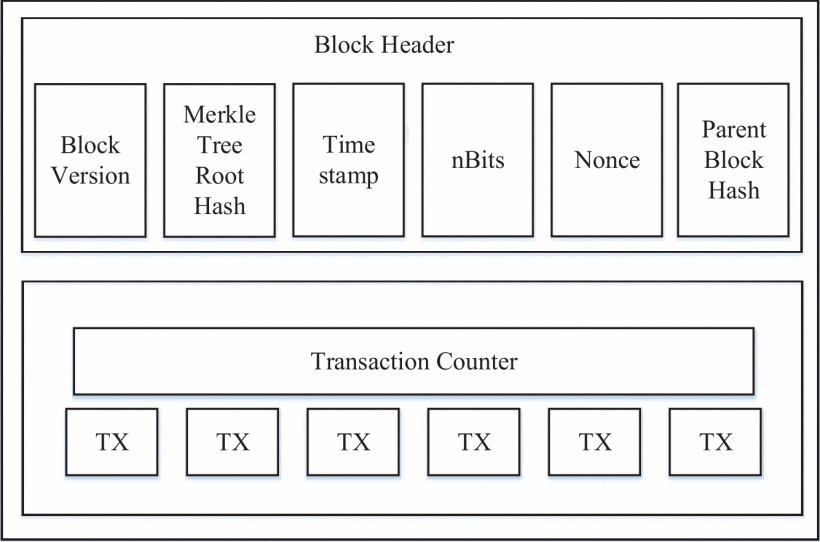
\includegraphics[width=0.75\textwidth]{obrazky-figures/block_schema.png}
	\caption{Schéma bloku \cite{blockchain_architecture1}.}
	\label{pic_block_schema}
\end{figure}

Telo bloku obsahuje jednotlivé transakcie uložené v~blockchaine. Integrita transakcií je zabezpečená jednak ich permanentným uchovaním v~rámci siete ale aj pomocou asymetrickej kryptografie a to použitím digitálneho podpisu. Užívateľom na vykonanie transakcie stačí mať vygenerovaný svoj unikátny verejný a súkromný kľúč. Súkromný je udržiavaný v~tajnosti a používa sa na podpisovanie transakcií, zatiaľ čo verejný slúži pre overenie autenticity transakcie. Transakcie podpísané súkromným kľúčom sú propagované do celej siete blockchainu, kde sú následne validované. Proces validácie prebieha prostredníctvom participujúcich sa výpočtových uzlov, ktoré rozhodujú pomocou konsenzus protokolu o~pravosti transakcie a jej následnom pridaní do blockchainu. Ak výpočtové uzly úspešne validujú autenticitu transakcie, tak ju zároveň aj pridajú do aktuálne vytváraného bloku. Pre zaistenie schopnosti uzla overiť validitu transakcie musí každý uzol uchovávať kópiu celého blockchainu. Využite asymetrickej kryptografie poskytuje vysokú dávku anonymity, nakoľko užívatelia sú identifikovateľní jedine svojím verejným kľúčom.

Z~hľadiska početnosti a príslušnosti participujúcich sa uzlov vieme blockchainy rozdeliť do troch kategórií, ktoré sa líšia v~efektivite, dostupnosti, miere zaručenia integrity i v~miere decentralizácie \cite{blockchain_architecture1}.

\begin{figure}[hbt]
	\centering
	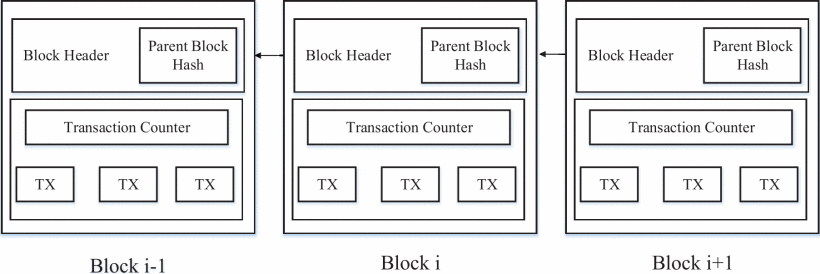
\includegraphics[width=\textwidth]{obrazky-figures/blockchain_scheme.png}
	\caption{Schéma blockchainu \cite{blockchain_architecture1}.}
	\label{pic_blockchain_scheme}
\end{figure}

\paragraph{Verejné}

Verejné blockchainové siete sú dostupné každému bez rozdielu, výpočtové uzly sa môžu samovoľne pripájať a podieľať sa na validácii autenticity transakcií. Transakcie s~overenou validitou a ich história sú vo verejnom blockchaine dostupné každému. Otvorená povaha sa javí ako lákavá pre nových užívateľov, čo pozorujeme na raste populárnych verejných blockchainov. Veľké množstvo výpočtových uzlov ale znamená, že propagovanie a validácia nových transakcií v~rámci siete zaberá značné množstvo času. Toto oneskorenie a limitovaná priepustnosť transakcií sú značnou nevýhodou verejného blockchainu. Veľký počet zapojených výpočtových uzlov má však aj svoje výhody, najmä vyššiu mieru integrity transakcií a tým pádom aj samotného blockchainu. Nakoľko na procese validácie sa podieľajú všetky výpočtové uzly, manipulácia s~transakciami uloženými v~rámci siete je v~prípade verejných blockchainov takmer nemožná.

\paragraph{Súkromné}

Sú plne kontrolované jednou autoritou, tým pádom sú do určitej miery centralizované a prispôsobené pre jej potreby. Prístup do súkromných blockchainov môže byť umožnený aj verejnosti, no vždy je spravovaný kontrolnou autoritou. Určenie spôsobu overovania validity transakcií je taktiež v~plne na rozhodnutí kontrolnej autority, typicky však na rozdiel od verejných blockchainov, transakcie validuje iba určitá skupina participujúcich sa uzlov. Toho prispieva aj ku ďalšej oblasti, kde majú súkromné blockchainy navrch, a tou je efektivita. Optimalizácia procesu validácie transakcií má za následok túto vysokú efektivitu, ktorá je spravidla vyššia než u~verejných blockchainov. Čo však tento typ blockchainu získa na efektivite naopak zase stratí na integrite. Súkromný blockchain umožňuje svojej kontrolnej autorite dohľad nad počtom uzlov a spôsobom validácie. Úplná kontrola nad týmito aspektami otvára teoretickú možnosť spätnej manipulácie s~už overenými transakciami.

\paragraph{Konzorcium blockchainy}

Nachádzajú sa na pomedzí súkromných a verejných blockchainov, čo platí aj o~ich vlastnostiach, výhodách a nevýhodách. Sú spravované viacerými autoritami, tým pádom majú  o~málo vyššiu mieru decentralizácie i integrity než súkromné blockchainy. Spôsob validácie transakcií zväčša býva rovnaký ako pri súkromných, čiže sa na nej podieľajú iba niektoré výpočtové uzly. V~súčasnosti sa vývojom konzorcium blockchainov zaoberá napríklad projekt Hyperledger \cite{hyperledger}.

\section{Konsenzus protokoly}

V~každom blockchaine môže nastať situácia, kedy sa výpočtový uzol, prípadne skupina, bude snažiť propagovať blok obsahujúci neplatné transakcie. Môže sa jednať o~chybu no aj o~zámer nelegitímneho uzla. Ak sa tak stane, je úlohou ostatných legitímnych a správne fungujúcich uzlov vzájomne dospieť k~dohode a nedovoliť propagáciu neplatného bloku. Vzhľadom na relatívnu anonymitu uzlov vo verejnom blockchaine, sa z~dosiahnutia dohody stáva netriviálny problém. Problematiku dosiahnutia dohody medzi výpočtovými uzlami v~nedôveryhodnom prostredí riešia takzvané konsenzus protokoly. Popisujú spôsob validácie transakcií ako aj to, ktoré uzly ju budú vykonávať. Vzhľadom na otvorenosť blockchainu je potrebné aplikovať správny konsenzus protokol. Ten je pre každý blockchain špecifikovaný v~Genesis bloku. Na konsenzus protokol sú kladené vysoké nároky vzhľadom na to, že jednou z~kľúčových vlastností blockchainu je decentralizácia, ktorá je zaručená práve schopnosťou uzlov dospieť k~vzájomnej korektnej dohode bez zásahu vyššej autority. Pomocou konsenzus protokolu taktiež jednotlivé výpočtové uzly preukazujú svoju legitimitu, väčšinou pomocou poskytnutia prostriedkov alebo protihodnoty. Schopnosť konsenzus protokolu správne fungovať aj pri výskyte neznámeho počtu chybne pracujúcich uzlov v~sieti sa nazýva odolnosť voči Byzantským chybám. Názov pochádza z~analógie problému Byzantských generálov \cite{byznatine_generals}. Najrozšírenejšie protokoly budú priblížené v~nasledujúcej časti \cite{blockchain_consensus}.

\paragraph{Dôkaz prácou - PoW (Proof of Work)}

Pri tomto protokole uzol propaguje blok vyriešením netriviálneho výpočtového problému. Jeho vyriešením dokazuje, že vykonal prácu. Po jeho vyriešení spropaguje výsledok do siete a ostatné uzly overia jeho správnosť a pripoja daný blok do svojej lokálnej kópie blockchainu. Výpočtový problém je navrhnutý tak aby jeho vyriešenie bolo výpočtovo zložité, no overenie jednoduché. Po vytvorení bloku súťažia participujúce sa uzly vo vyriešení výpočtového problému. Uzol, ktorému sa to ako prvému podarí, propaguje riešenie do siete aby ho ostatné uzly mohli overiť. Motiváciou pre vynaloženie značných prostriedkov na riešenie výpočtového problému je odmena, zväčša v~podobe určitého obnosu kryptomeny, poskytovanej daným blockchainom.

Príkladom výpočtového problému a jeho riešenia je nájdenie takého hešu hlavičky bloku, ktorý splňuje určité kritérium, spravidla také, ktoré obmedzuje dĺžku výsledného hešu. Variabilita výsledného hešu spočíva v~čísle nonce (number only used once), ktoré je pripojené ku hlavičke bloku pred vypočítaním jej hashu. Jednotlivé uzly medzi sebou súťažia a snažia sa nájsť také číslo nonce aby výsledný heš spĺňal zadané kritérium. Pre nájdenie tohto čísla je potrebné veľké množstvo spočítaní hešu hlavičky, čo je výpočtovo náročné. Kritérium pre dĺžku výsledného hešu sa s~pribúdajúcim množstvom blokov v~blockchaine znižuje, čím sa zvyšuje zložitosť problému. Zvyšovanie zložitosti výpočtového problému je nevyhnutné pre zaistenie decentralizovanej povahy blockchainu.

V~Blockchaine pracujú výpočtové uzly nezávisle nakoľko ide o~distribuovanú sieť. Toto môže viesť k~situácii kedy viaceré uzly nájdu riešenie v~rovnaký čas, čo má z~následok tvorbu vetví v~rámci reťazca blokov. Vetvenie v~blockchaine znázornené na obrázku \ref{pic_block_fork} V~tomto prípade sú platné oba bloky, no v~tomto protokole je pravidlom, že uzly pokračujú v~najdlhšej im známej vetve. Kratšie vetvy sú následne opustené.

Tento protokol sa využíva najmä vo verejných blockchainoch, pretože kladie dôraz na celkový výpočtový výkon namiesto na počet participujúcich sa uzlov.

\paragraph{Dôkaz vkladom – PoS (Proof of Stake)}

Protokol založený na predpoklade, že čím väčší má používateľ podiel v~blockchaine, tým menšia je pravdepodobnosť, že sa ho pokúsi napadnúť. Pod podielom, respektíve vkladom sa rozumie istá časť kryptomeny v~danom blockchaine, ktorá je po dobu vytvárania bloku daným uzlom uzamknutá. Tento protokol nevyžaduje intenzívne výpočty ani súťaženie medzi jednotlivými uzlami. Uzol poverený vytváraním nasledujúceho bloku je vybraný podľa pomeru vkladu daného uzla voči celkovému objemu kryptomeny v~blockchaine. Metód pre výber je niekoľko.

Výber uzla vytvárajúceho blok môže byť náhodný, pričom sieť sa pozrie na veľkosť vkladu každého uzla a z~neho určí percentuálnu šancu pre na to aby bol daný uzol vybraný. Percentuálna šanca je rovná pomeru vkladu uzla ku celému objemu kryptomeny v~danom blockchaine.

Pri výbere uzla a bloku vo viackolovom výberovom procese sa na začiatku vyberie niekoľko uzlov, z~ktorých každý z~nich vytvorí jeden blok. Následne každý uzol, ktorý má vykonaný vklad, hlasuje o~tom, ktorý blok bude pripojený do blockchainu. Hlasovanie sa môže udiať vo viacerých kolách a dáva všetkým užívateľom bez rozdielu výšky vkladu možnosť hlasovať o~pripojení nasledujúceho bloku.

Pri výbere uzla podľa času uplynutého od vkladu je nevyhnutné aby blockchain disponoval záznamom o~čase vloženia vkladu. V~tomto prípade systém pripisuje uzlu šancu vytvoriť nasledujúci blok podľa jeho vkladu no až po uplynutí určitého času od jeho vykonania. Po tom, ako je uzol vybraný a vytvorí blok, sa záznam o~uplynutom čase od vloženia jeho vkladu vynuluje, čím sa efektívne vynuluje aj šanca uzla na to aby bol znova vybraný. Táto šanca sa opäť obnoví po uplynutí určitého času. Ten spôsob výberu stále výrazne zvýhodňuje uzly s~vyšším vkladom, no zamedzuje im dominanciu nad systémom.

Pri výbere uzla pomocou voľby delegátov participujúce uzly hlasujú o~to, ktoré uzly budú vytvárať nové bloky. Váha každého hlasu je úmerná vkladu daného uzla. Uzly s~najväčším počtom hlasov následne vytvárajú nové bloky. Hlasovať je možné aj za odstránenie daného uzlu zo skupiny, ktorá vytvára bloky. Hlasovanie je kontinuálny proces čo znamená, že uzly sa snažia korektným správaním udržať sa v~skupine tvorcov blokov, aby neprišli o~odmenu. 

Výhodou tohto protokolu oproti dôkazu prácou je najmä násobne nižšia náročnosť na výpočtový výkon a s~ním spojené faktory. Napriek tomu je však vhodný pre využitie v~nedôveryhodnom prostredí, teda vo verejných blockchainoch.

\begin{figure}[hbt]
	\centering
	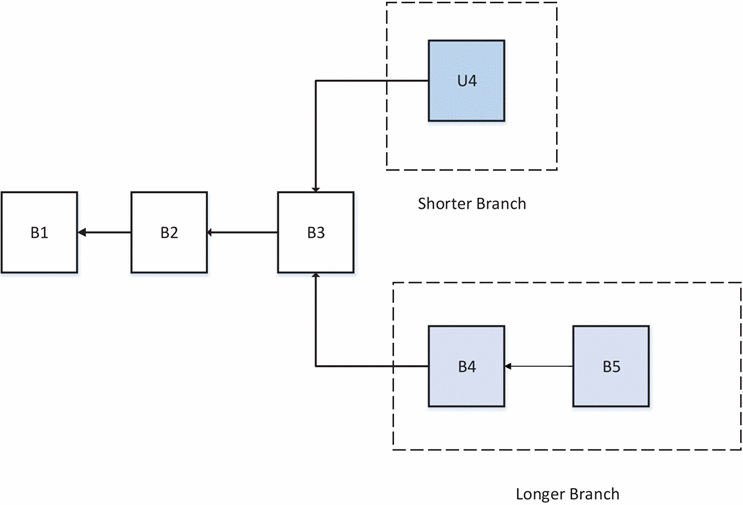
\includegraphics[width=0.75\textwidth]{obrazky-figures/block_branch.png}
	\caption{Vizualizácia vetvenia v~blockchaine \cite{blockchain_architecture1}.}
	\label{pic_block_fork}
\end{figure}

\paragraph{Dôkaz autority  - PoA (Proof od Authority)}

Jedná sa o~protokol zameraný pre použite v~súkromných blockchainoch. Jeho koncept pochádza z~praktík využívaných v~architektúre distribuovaných systémov. Pracuje s~N dopredu určenými autoritatívnymi uzlami, z~ktorých má každý svoj unikátny identifikátor. Tieto autoritatívne uzly následne vykonávajú konsenzus protokol nad transakciami prichádzajúcimi od klientov. Ten pracuje na princípe pravidelného striedania vedúceho uzla, pričom ten ako jediný v~danom momente vytvára následujúci blok. Po vytvorení a spropagovaní bloku do siete aktuálnym vedúcim uzlom sa vyberie nový vedúci a celý proces vytvárania bloku začína odznova. Striedanie role vedúceho uzla vytvárajúceho bloky zároveň zaručuje rovnomerné rozdelenie výpočtovej práce medzi participujúce sa uzly.

V~tomto ohľade je tento protokol efektívnejší než vyššie spomínané PoW alebo PoS. Slabé miesto tohto protokolu však spočíva v~potrebe vzájomnej dôvery medzi uzlami. Pre správne fungovanie siete je potrebné aby aspoň N/2 + 1 bolo skutočne dôveryhodných. Z~tohto dôvodu tento protokol nie je vhodný pre blockchainy s~voľným prístupom do siete.

\paragraph{Practical Byzantine Fault Tolerance - PBFT}

Protokol mierne podobný s~PoA, tolerujúci maximálne jednu tretinu škodlivých uzlov. Proces dosiahnutia konsenzusu začína náhodným výberom vedúceho uzla, ktorý v~danom kole zhromažďuje transakcie a vytvára z~nich jeden celistvý blok. Po nazhromaždení dostatočného množstva transakcií na vytvorení jedného bloku vyšle vedúci uzol do siete správu pre ostatné uzly, ktorá značí začiatok tvorby bloku. Tie po jej prijatí začnú sami simulovať vytváranie bloku. Po jej dokončení každý uzol vyšle do siete ďalšiu správu, slúžiacu na overenie autenticity transakcií v~aktuálne vytváranom bloku. Po prijatí 2f+1 správ potvrdzujúcich autenticitu bloku, (pri predpoklade, že celkový počet participujúcich sa uzlov je 3f), vyšle uzol správu všetkým ostatným uzlom, ktorou signalizuje svoju pripravenosť na pridanie vytváraného bloku do blockchainu. Následne po prijatí 2f+1 správ o~pripravenosti na prijatie je daný blok pridaný do lokálnej kópie blockchainu daného uzla. Týmto proces pridávania bloku končí \cite{pbft}.

Nevýhodou tohoto protokolu je nízka škálovateľnosť nakoľko pre propagáciu každého uzla je potrebná výmena minimálne dvoch správ medzi všetkými uzlami. Taktiež, v~prípade že sa vedúci uzol pokúsi spropagovať nelegitímny blok, systém to odhalí a blok sa nevytvorí, čím bude ovplyvnená efektivita blockchainu.


\paragraph{Dôkaz identity - PoR (Proof of Reputation)}

Využívaný hlavne v~blockchainoch s~kontrolovaným prístupom a zaručenou určitou mierou dôvery. Každý uzol, ktorý má záujem o~vytváranie blokov musí mať preukázateľne prepojenú svoju identitu v~rámci blockchainu s~identitou z~reálneho sveta. Zároveň musí byť toto prepojenie overené autoritou a dostupné ostatným uzlom v~sieti. Uzol vytvorením bloku dáva do stávky svoju reputáciu, ktorú mu hodnotia ostatné uzly v~rámci siete. Tá sa môže znížiť ak uzol nekoná v~súlade s~pravidlami blockchainu, alebo naopak zvýšiť ak je ním vykonaná práca korektná. Čím vyššiu má uzol reputáciu, tým je vyššia šanca, že mu sieť dovolí vytvoriť blok. Tým pádom je v~záujme uzla držať si vysokú reputáciu.

\paragraph{Dôkaz uplynutého času - PoET (Proof of Elapsed Time)}

Pri tomto type protokolu uzly vytvárajú blok po uplynutí náhodného časového intervalu. Každý uzol si najprv vyžiada od svojho dôveryhodného hardvérového modulu náhodnú hodnotu, ktorá predstavuje dobu, po ktorú bude uzol čakať kým vytvorí blok. Uzol, ktorý sa ako prvý prebudí následne vytvorí blok a zobudí ostatné, uspané uzly. Je však potrebné vedieť overiť, že uzol naozaj počkal náhodnú dobu pred vytvorením bloku. O~toto sa stará dôveryhodný hardvérový modul, ktorý po uplynutí danej doby poskytne uzlu podpísaný certifikát, ktorý uzol následne zverejní spolu s~vytvoreným blokom.


\chapter{Centralizovaná a decentralizovaná autentifikácia}

V~tejto kapitole bude porovnaný centralizovaný a decentralizovaný prístup ku autentifikácii. Poznatky v~tejto kapitole boli čerpané z~\cite{auth_sys_comparison}.

S~rozšírením možností internetu vznikla pre vykonávanie mnohých úkonov v~kyberpriestore potreba autentifikovať jednotlivé entity pomocou digitálnej identity. Pod pojmom entita rozumieme osobu, organizáciu, hardvérové zariadenie alebo aj softvérový program. Digitálna identita obsahuje prostriedky, vo forme informácií, ktoré reprezentujú určitú entitu a pomocou ktorých je možné ju vyhodnotiť a autentifikovať bez manuálneho zásahu. Formy digitálnej identity sa líšia najmä v~spôsobe, akým sú spravované.

\section{Centralizované}

Pri toto modeli prevádzkuje systém digitálnej identity poskytovateľ služby, ktorá autentifikáciu vyžaduje. Poskytovateľ služby spravuje identitu a všetky relevantné dáta registrovaných používateľov. Jedná sa o~v~súčasnosti najrozšírenejší model správy identity, používaný širokou škálou poskytovateľov rôznych služieb, pričom autentifikačné prostriedky majú väčšinou podobu prihlasovacieho mena a hesla. Samotná digitálna identita je uložená v~databáze prevádzkovateľa služby, pričom jej rozsah a kvalita závisí od typu služby, pre ktorý sprostredkováva autentifikáciu.

Nevýhodami tohoto modelu z~používateľského hľadiska sú najmä nulová kontrola nad vlastnými dátami, nakoľko sú spravované treťou stranou, a potreba veľkého množstva používateľských účtov pre služby od rôznych poskytovateľov. Z~hľadiska poskytovateľa sa ako nevýhody javia náklady spojené s~uložením, udržiavaním a ochranou používateľských dát. Najmä v~prípade ochrany môže byť poskytovateľ zákonne povinný zabezpečiť predpísanú mieru ochrany a spôsob manipulácie s~dátami užívateľov, ako tomu je v~rámci európskej smernice GDPR.

\section{Federatívne}

Ide o~spojenie viacerých centralizovaných systémov správy identity. Toto je možné docieliť ak systémy využívajú rovnaký štandard ako tomu je napríklad pri cestovných dokladoch v~rámci Európske únie, alebo ak sa správcovia dohodnú na vzájomnom akceptovaní svojich systémov. Pre zaistenie spolupráce systémov rôznych štandardov je potrebné vykonať právne a technické kroky, čo so sebou môže niesť nemalé náklady. Taktiež, nakoľko sa jedná o~centralizovanú architektúru, ich kvalita a dôveryhodnosť sa môže dramaticky líšiť systém od systému. Z~používateľského javiska je výhodné vedieť sa autentifikovať pomocou jednej identity do služieb od rôznych poskytovateľov. Príkladom systému federatívnej identity je API poskytované protokolom OAuth\footnote{\url{https://oauth.net/2/}}, ktorý využívajú aj Facebook a Google. Nevýhodou pre používateľov je opäť nulová kontrola nad vlastnými údajmi a možnosť sledovania ich aktivity naprieč rôznymi službami.

\section{Decentralizované}

Entita sama zodpovedá za vytvorenie, uloženie, správu a distribúciu svojej digitálnej identity. Pre jej reprezentáciu sa používa, decentralizovaný identifikátor (DID), ktorý pozostáva z~verejného a súkromného kľúča. Verejná časť DID je uložená takým spôsobom, aby bola zaručená jej integrita, dostupnosť, nemennosť a auditovateľnosť. Zvyšné súčasti digitálnej identity tvoria digitálne poverenia, ktoré sú uložené v~súkromnom úložisku entity, zväčša sa jedná o~počítač, mobil alebo cloudové riešenie. Entita si má následne plnú kontrolu nad získanými digitálnymi povereniami (Verifiable Credentials) a tie využíva pri autentifikácii podľa potreby. Jednotná podoba tohto modelu zatiaľ nie je nakoľko sa do praxe dostal iba v~obmedzenom rozsahu.

\subsection{Príklady konceptov}
V~prípade protokolu pre decentralizovaný autentifikačný systém, navrhnutom v~\cite{dec_auth1} je uloženie samotných dát plne v~réžii užívateľa, pričom samotná identita v~podobe DID je z~dôvodu dôveryhodnosti uložená v~blockchaine. Problematiku ochrany biometrických údajov tento protokol rieši za použitia štandardu BOPS \cite{ieee_bops}, teda rozdelením miesta ich uloženia medzi zariadenie užívateľa a vzdialený server. Biometrická autentifikácia následne môže prebiehať lokálne aj na vzdialenom serveri.

Mierne podobný prístup využíva systém navrhnutý v~\cite{dec_auth2}. Pri zápise užívateľa je jeho biometrická šablóna rozdelená a niekoľko kópií fragmentov je uložených medzi náhodne vybrané klientske stanice systému, pričom údaj tom, ktoré to sú je uložený do blockchainu. Následne počas autentifikácie je pomocou smart kontraktu z~blockchainu získaná informácia o~miestach uloženia jednotlivých častí šablóny. Tie sú zo systému stiahnuté na klientsku stanicu, kde aj prebehne ich rekonštrukcia a porovnanie so vstupnou šablónou.

Posledným príkladom je systém navrhovaný v~\cite{dec_auth3}, kde je identita reprezentovaná kľúčovým párom, ktorý je spravovaný dôveryhodným hardvérovým modulom. Užívateľ následne komunikuje, pomocou aplikácie s~webovým serverom konkrétnej služby, u~ktorého sa potrebuje autentifikovať. Samotné prvky identity pre jednotlivé služby sú opäť uložené v~blockchaine. Pri pokuse o~autentifikáciu webový server v~blockchaine podľa verejného kľúča vyhľadá údaje relevantné pre danú službu.


\section{Porovnanie}
Rozdiely medzi týmito prístupmi sa dajú rozdeliť do viacerých kategórií. Z~hľadiska správy identity a dát užívateľov dáva centralizovaný prístup túto zodpovednosť plne do rúk poskytovateľa služby. Ten rozhoduje o~spôsobe ich uloženia a ochrany. Dáta sa taktiež jednoduchšie môžu dostať do rúk tretích strán, buď z~iniciatívy samotného poskytovateľa služby alebo, v~krajnom prípade, zlyhaním zabezpečenia ich úložiska. Centralizované riešenia sú náchylnejšie voči útokom, nakoľko miesto ich správy a uloženia je zväčša sústreďované do jedného bodu. Naopak v~prípade decentralizovaných riešení má užívateľ určitú formu kontroly nad zabezpečením a/alebo spôsobom uloženia svojich údajov.

Z~hľadiska jednoduchosti prevedenia a užívateľskej prívetivosti má v~súčasnej dobe centralizovaný prístup navrch. Nakoľko celý systém správy identity je pod kontrolou jednej entity, tá si ho môže sama navrhnúť a modifikovať podľa svojich aktuálnych potrieb. Mnohé centralizované riešenia súčasnosti poskytujú užívateľom možnosť autentifikovať sa u~viacerých poskytovateľov služieb pomocou jedného systému, čo sa javí ako prívetivé. V~prípade decentralizovaného prístupu v~súčasnej dobe nie je v~praxi zavedený univerzálne akceptovaný štandard. \cite{identity_comparison} 


\chapter{Návrh systému}
Táto kapitola rozoberá návrh decentralizovaného biometrického autentifikačného systému schopného detekcie porušenia integrity dátového úložiska biometrických šablón. Taktiež budú priblížené jeho jednotlivé časti a ich vstupy, výstupy a fungovanie. Snahou je navrhnúť systém tak, aby boli úkony spojené s~autentifikáciou decentralizované, prípadne tak aby poskytoval kontrolné mechanizmy pre svoje centralizované časti.

Systém bude slúžiť na zápis a následnú autentifikáciu užívateľa pomocou odtlačku prsta. Užívateľ sa bude v~rámci systému identifikovať pomocou verejného kľúča. Systém poskytne užívateľovi kontrolu nad zabezpečením vlastných biometrických dát, ktoré budu pred uložením do databázového systému šifrované jeho verejným kľúčom. Toto zabezpečí, že v~prípade úniku dát z~databázového systému budú údaje naďalej chránené spôsobom, ktorého prostriedky sú čisto v~réžii užívateľa. Nakoľko databázový systém je sám o~sebe centralizovaný, systém obsahuje mechanizmus pre kontrolu jeho integrity. Ten bude spočívať v~uložení dôveryhodnom uložení kryptografického odtlačku dát ukladaných do databázy. Zároveň s~ich uložením bude zároveň aj ich kryptografický odtlačok uložený do blockchainu pomocou smart kontraktu. Tento odtlačok bude pri pokuse o~autentifikáciu z~blockchainu získaný a porovnaný s~odtlačkom zhotoveným z~dát pochádzajúcich z~databázy. Pred porovnaním je šablóna za databázy dešifrovaná. Celý proces zápisu a autentifikácie t.j. snímanie biometrickej šablóny, jej následné šifrovanie a dešifrovanie, vytváranie kryptografických odtlačkov a porovnávanie šablón bude vykonávané lokálne, v~klientskej aplikácii. Fyzické usporiadanie systému je znázornené na obrázku \ref{pic_system_physical}

Biometrická autentifikácia s~dodatočnou nutnosťou využitia tajného kľúča sa môže zdať ako neprívetivá z~pohľadu užívateľa. Tento spôsob bol však zvolený pre zvýšenie zabezpečenia biometrických údajov užívateľa a zároveň pre naplnenie decentralizovanej podstaty systému.

\begin{figure}[hbt]
	\centering
	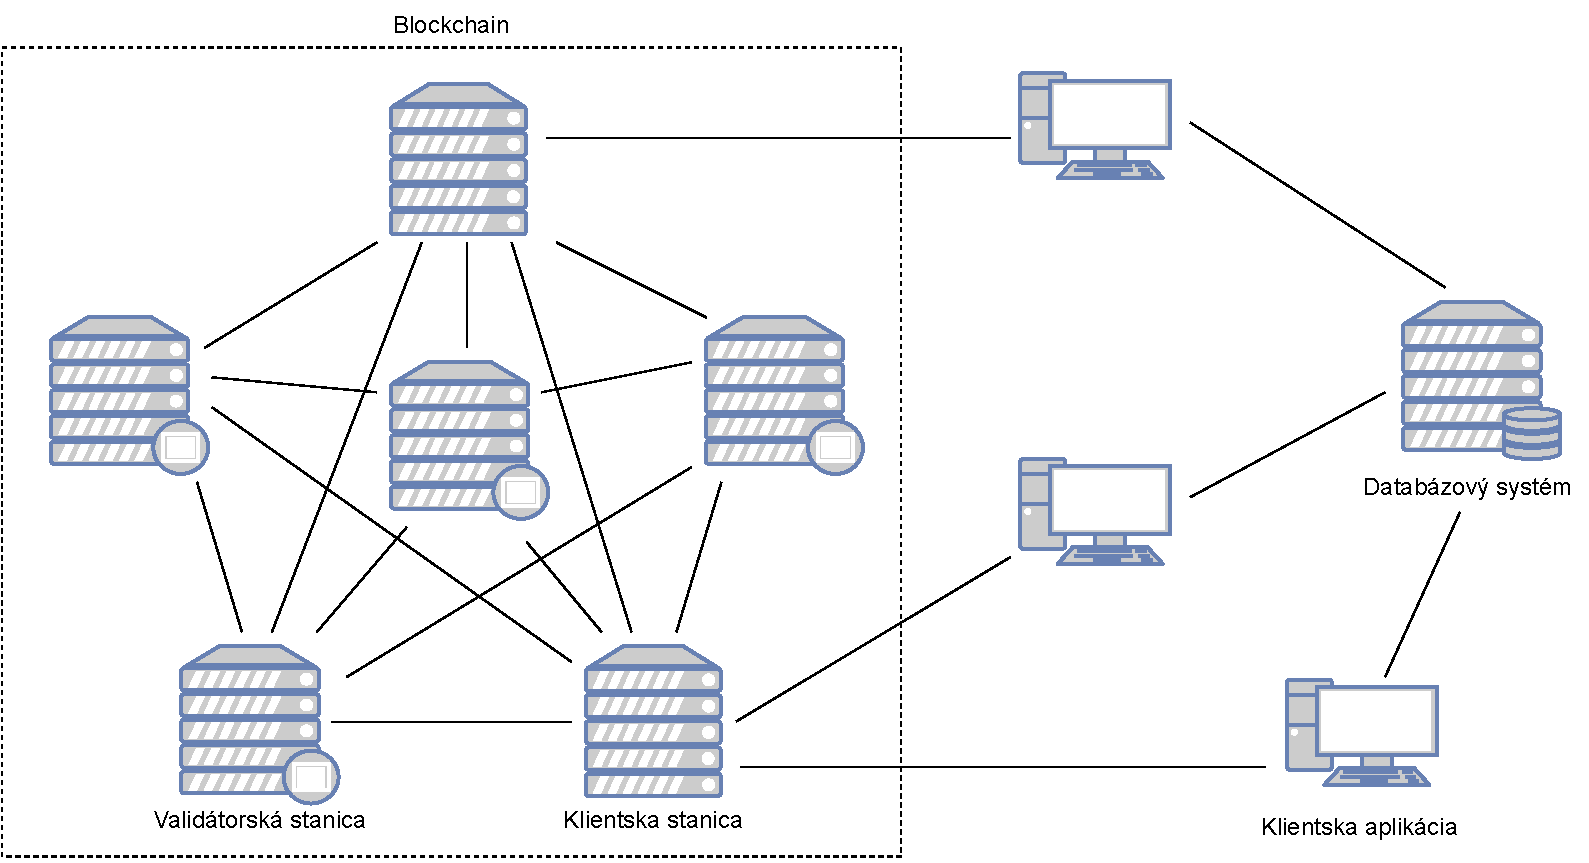
\includegraphics[width=\textwidth]{obrazky-figures/physical_sys.pdf}
	\caption{Fyzická schéma systému.}
	\label{pic_system_physical}
\end{figure}

\section{Architektúra systému}
Systém sa skladá z~niekoľkých hlavných častí, ktoré môžeme vidieť na obrázku \ref{pic_navrh}. Prvou z~nich je biometrický senzor, ktorý sníma odtlačky prsta a následne z~nich produkuje biometrické šablóny. Tie spracováva a zabezpečuje nasledujúci, transformačný, modul. Transformovanú šablónu následne prevezme hlavný modul, ktorý reprezentuje klientskú aplikáciu. Ten jednak slúži na jej zabezpečenie pred ďalším uložením a zároveň sa stará o~jej predávanie do a z~databázy a o~nahrávanie jej kryptografického odtlačku do blockchainu.

\begin{figure}[hbt]
	\centering
	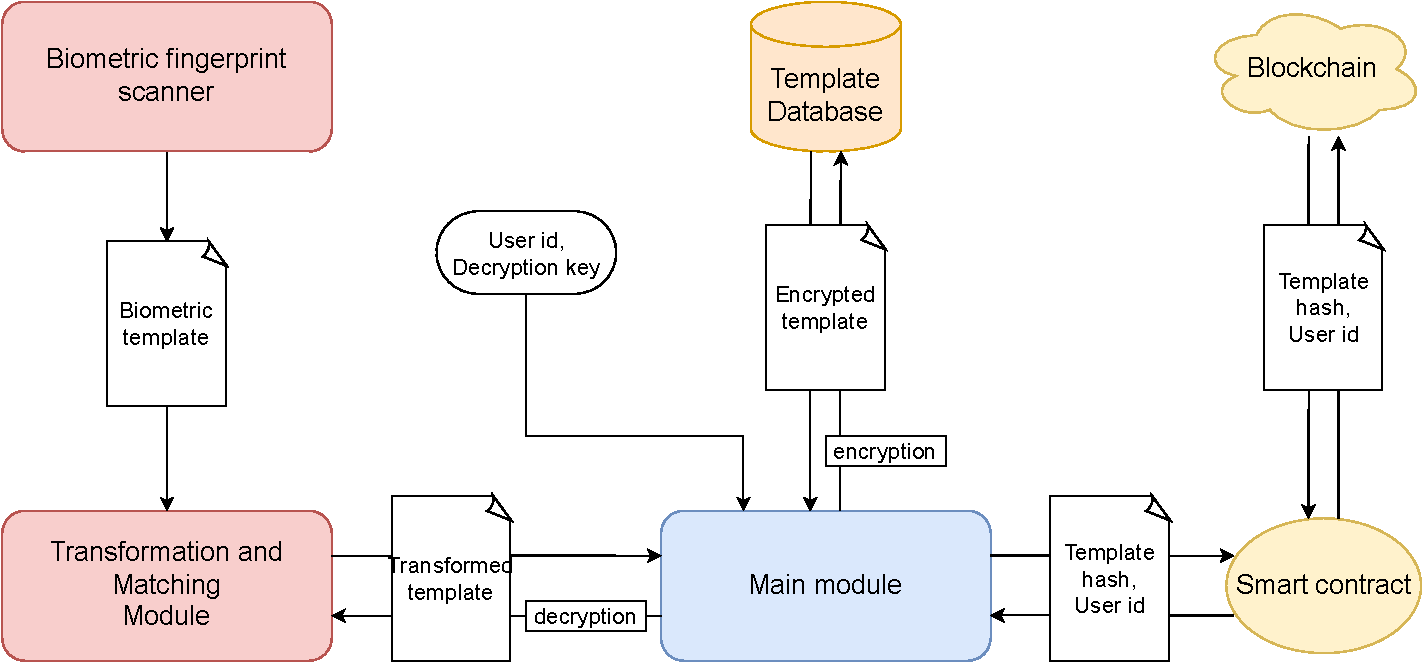
\includegraphics[width=\textwidth]{obrazky-figures/navrh.pdf}
	\caption{Schéma návrhu systému.}
	\label{pic_navrh}
\end{figure}

\section{Biometrický senzor a Transformačný modul}
Pre potreby nasnímania odtlačku prsta bude postačovať kapacitný alebo optický senzor. Musí však disponovať možnosťou uloženia nasnímaných biometrických dát mimo svoj dôveryhodný hardvérový modul. Uloženie biometrických dát v~dôveryhodnom hardvérovom module poskytuje vyššiu mieru zabezpečenia, no pre potreby navrhovaného systému, najmä autentifikácie z~viacerých lokalít, jeho použitie nie je možné. Systém ďalej predpokladá prácu s~biometrickou šablónou reprezentovanou vo formáte určenom štandardom ISO/IEC 19794-2 \cite{ISO19794-2} o~maximálnej veľkosti 1566 bajtov.

V~rámci transformačného modulu budú šablóny zabezpečené pomocou ireverzibilnej transformačnej funkcie, tak aby z~nich nebolo možné zrekonštruovať pôvodný odtlačok prsta \cite{template_transform}. Vstupom tejto funkcie je kľúč, ktorý bude v~prípade navrhovaného systému spravovať užívateľ. Porovnávanie samotných odtlačkov prstov tým pádom bude prebiehať v~transformovanej doméne. Celý tento proces je znázornený na obrázku \ref{pic_transform} Výstupom transformačného modulu je transformovaná biometrická šablóna uložená vo formáte danom štandardom ISO/IEC 19794-2.

\begin{figure}[hbt]
	\centering
	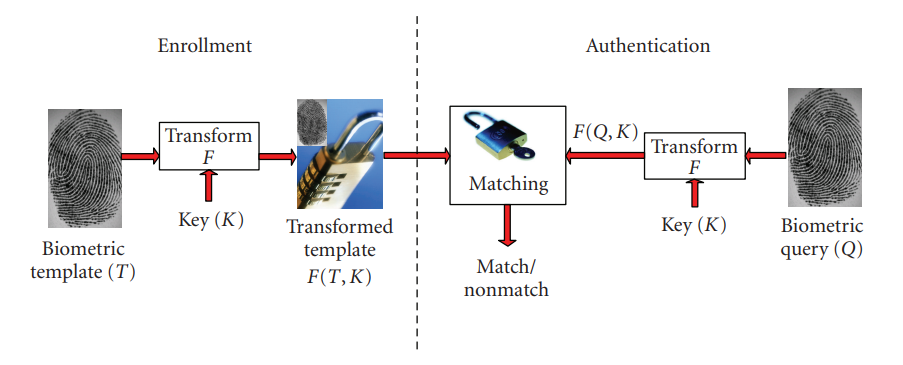
\includegraphics[width=\textwidth]{obrazky-figures/transform.png}
	\caption{Schéma transformácie v~systéme \cite{template_security}.}
	\label{pic_transform}
\end{figure}

\section{Hlavný modul}

\subsection{Správa užívateľov}
Z~podstaty systému bude potrebné nejakým spôsobom vedieť užívateľov identifikovať. Taktiež musí každý užívateľ disponovať prostriedkom pre zabezpečenie svojej biometrickej šablóny. Pre naplnenie oboch týchto potrieb bol zvolený systém súkromných a verejných kľúčov. Na základe poznatkov a záverov z~\cite{keyselect} boli zvolené kľúče spĺňajúce štandard PKCS\#1 o~veľkosti 2048 bitov. Verejný kľúč bude slúžiť ako jedinečný identifikátor používateľa, a zároveň šifrovací kľúč pre neskôr použitý šifrovací algoritmus.

\subsection{Zabezpečenie}
Po prechode biometrickej šablóny transformačným modulom sa zvýši jej bezpečnosť, no stále ide o~veľmi citlivé dáta. Tu vzniká potreba zabezpečenia v~podobe šifrovania pred jej ďalším uložením. Cieľom zároveň je, aby následné dešifrovanie šablóny bolo možné iba so spoluprácou užívateľa. Pre tento účel sa javí ako najlepšia voľba hybridná šifra , t.j. asymetrická šifra v~kombinácii so symetrickou. Je nutné použiť oba druhy šifier, nakoľko asymetrickú šifra nie je vhodná pre zabezpečenie väčších súborov.

Hybridná šifra zároveň poskytuje kombináciu výhod oboch druhov šifier a to rýchlosť a efektivitu symetrickej šifry s~pohodlnosťou a užívateľskou prívetivosťou asymetrickej šifry. Pre asymetrickú šifru bol zvolený algoritmus RSA, ktorý ako šifrovací kľúč využívať verejný kľúč užívateľa. Samotná šablóna bude zašifrovaná symetricky, pomocou algoritmu AES. Symetrický šifrovací kľúč dĺžky 128 bitov bude náhodne vygenerovaný pri každom šifrovaní. Po použití bude zašifrovaný pomocou symetrickej šifry a následne pripojený ku šablóne. Takto zabezpečené dáta sú pripravené na opustenie systému, čiže. uloženie do dátového úložiska.


\subsection{Dátové úložiská}
V~systéme sú potrebné dve dátové úložiská, každé s~rôznym účelom a požiadavkami. Hlavné úložisko bude slúžiť pre ukladanie šifrovaním zabezpečených biometrických šablón. Požiadavkami na hlavné úložisko sú vysoká rýchlosť prístupu a možnosť uložiť dáta vo veľkosti približne 2,5 kilobajtov na užívateľa. Sekundárne úložisko bude slúžiť na ukladanie kryptografických odtlačkov dát ukladaných do hlavného úložiska. Pri sekundárnom úložisku hrá dôležitú úlohu najmä jeho dôveryhodnosť a auditovateľnosť, nakoľko na ňom bude stáť pridaná integrita systému.

\subsubsection{Hlavné úložisko - Databázový systém}
Pre uskladnenie zašifrovaných biometrických šablón bude použitý Open Source relačný databázový systém MySQL\footnote{\url{https://www.mysql.com/}} vo verzii 8.0. Pre jeho umiestnenie na sieti bude využitý databázový server firmy WebSupport\footnote{\url{https://www.websupport.sk/}}. Štruktúra databázového systému pozostáva z~jednej tabuľky, obsahujúcej 3 stĺpce. Jeden pre verejný kľúč používateľa, jeden pre zašifrované dáta a jeden pre identifikačné číslo záznamu. Pohyb dát do a z~databázového systému bude prebiehať pomocou SQL dotazov priamo z~klientskej aplikácie na databázový server.

\subsubsection{Sekundárne úložisko - Blockchain}
Funkciu sekundárneho úložiska bude v~navrhovanom systéme zastávať distribuovaná účtovná kniha (DLT), konkrétne blockchain Ethereum bežiaci v~privátnom nastavení. Jednotlivé stanice sa budú pracovať na princípe konsenzus protokolu PoA, konkrétne jednej z~jeho verzií pre Ethereum, Clique. Táto verzia bola vybraná pretože v~porovnaní s~ostatnými typmi konsenzus protokolov pre privátne blockchainy, najmä PBFT, poskytuje dobrú škálovateľnosť \cite{consensus_perf_comparison}.

\paragraph{Princíp algoritmu Clique}
Táto implementácia PoA poskytuje možnosť dynamického zoznamu autoritatívnych uzlov, aktuálne autoritatívne uzly môžu hlasovať o~pridaní alebo odobratí tohoto statusu. Samotný konsenzus protokol pracuje v~epochách, pričom pri začiatku každej epochy je do siete propagovaný špeciálny prechodný blok, ktorý okrem iných dát obsahuje aj opäť špecifikovaný zoznam autoritatívnych uzlov. Pri vytváraní aktuálneho bloku sa uzly, tak ako je v~PoA štandardom, striedajú.

Špecifikom Clique je fakt, že v~každom kole vytvárania bloku určeného na propagáciu protokol dovoľuje navrhovať bloky viacerým uzlom, no vždy iba jeden z~nich je tým vedúcim. Výber vedúceho uzla prebieha pomocou funkcie, ktorá berie do úvahy poradové číslo aktuálneho bloku a počet predom špecifikovaných autoritatívnych uzlov $N$. Každému uzlu je povolené propagovať iba každý $(N/2) + 1$-vý blok, čo znamená, že v~každom kole je iba $N-(N/2+1)$ blokom dovolená propagácia. Na začiatku kola je jednotlivým blokom od každého uzlu priradené skóre, pričom blok vytváraný lídrom má toto skóre najväčšie. Počas kola sa každý uzol okrem lídra pokúsi spropagovať svoj blok až po uplynutí náhodného časového intervalu, pričom líder sa snaží propagovať svoj blok hneď po jeho vytvorení. Tento mechanizmus zaručuje, že v~aj v~prípade ak líder nespropaguje blok, či už kvôli chybe alebo sa snaží zámerne uškodiť sieti, bude v~danom kole blok vytvorený jedným z~ostatných $N-(N/2+1)$ uzlov, pravdepodobne tým s~najnižším náhodným časovým intervalom. Táto periodicky rotujúca množina uzlov zaručuje odolnosť voči Byzantským chybám.

Avšak, vzhľadom na fakt, že v~rovnakom čase je v~sieti viacero tvorcov blokov môže nastať situácia kedy naraz dôjde ku propagácii viacerých blokov a blockchain sa rozvetví. Pre potlačenie a eventuálnu elimináciu tohto problému je Clique navrhnutý tak aby spolupracoval s~GHOST protokolom\footnote{\url{https://ethereum.org/en/whitepaper/##modified-ghost-implementation}} pre Ethereum. Ten zaručuje pokračovanie blockchainu vo vetve s~najvyšším skóre, čím zaručuje eventuálnu synchrónnosť siete. Protokol je využívaný hlavne v~sieťach s~nízkou dobou tvorby bloku, kde je vysoká šanca vetvenia.

\paragraph{Stanice v~sieti}
Stanice budú rozdelené do dvoch skupín. Prvou skupinou budú validátorské stanice, ktoré budú disponovať schopnosťou vytvárať a propagovať nové bloky. Druhú skupinu budú tvoriť klientske stanice, ktoré budú slúžiť na pripojenie do siete a spracovávanie požiadaviek pre zápis a čítanie z~blockchainu. Tieto klientske stanice budú bežať samostatne a hlavný systém sa na nich bude pripájať pomocou protokolu \texttt{http}. Tieto stanice budú taktiež disponovať obnosom blockchainovej meny potrebnej pre vykonávanie transakcií, ktoré spotrebúvajú Gas\footnote{\url{https://ethereum.org/en/developers/docs/gas/}}. Po vykonaní takejto transakcie sú pri konsenzus protokole PoA tieto prostriedky presunuté validátorskej stanici, ktorá podpísala blok obsahujúci danú transakciu. Pre zaistenie správneho chodu a dostupnosti systému bude potrebné tieto prostriedky dynamicky presúvať medzi validátorskými a klientskymi stanicami.

\subsection{Zaručenie integrity}
Ako už bolo spomenuté, systém disponuje zvýšenou mierou integrity v~podobe kontroly dát z~externého hlavného dátového úložiska. Vo fáze registrácie užívateľa sa zo zašifrovaných dát, obsahujúcich biometrickú šablónu, vytvorí kryptografický odtlačok, ktorý sa následne pomocou smart kontraktu uloží do sekundárneho úložiska, teda blockchainu. Systém vykoná počas procesu autentifikácie užívateľa kontrolu integrity zašifrovaných dát, ktoré získa z~databázy, porovnaním ich kryptografického odtlačku s~odtlačkom uloženým v~blockchaine. Vďaka auditovateľnosti blockchainu a použitiu eventu v~smart kontrakte je možné zistiť či sú tieto dáta autentické alebo či boli v~hlavnom úložisku nejakým spôsobom pozmenené a tým pádom skompromitované.


\chapter{Implementácia}
V~tejto kapitole sú popísané detaily implementácie jednotlivých častí systému a konkrétnych úkonov, ktoré vykonáva. Systém je určený pre operačný systém Windows 10. Hlavná časť systému bola napísaná v~programovacom jazyku Python vo verzi 3.9.12. Hlavné úložisko - databázový systém - využíva dotazy napísané v~jazyku SQL. Sekundárne úložisko - blockchain Ethereum - využíva pre implementáciu jednotlivých staníc nástroj Geth\footnote{\url{https://geth.ethereum.org/}} vo verzii 1.10.17 napísaný v~programovacom jazyku Go. Pre napísanie smart kontraktu bol využitý objektovo orientovaný jazyk Solidity\footnote{\url{https://docs.soliditylang.org/en/v0.8.13}}.

\section{Transformačný modul a porovnanie odtlačkov}
Pre zjednodušenie implementácie nie sú tieto moduly implementované. Pre demonštráciu funkčnosti kľúčových vlastností systému sú autentické biometrické šablóny nahradené náhodnou sekvenciou bajtov rovnakej dĺžky, akú predpisuje systémom predpokladaný štandard uloženia biometrických šablón ISO/IEC 19794-2.

\section{Hlavný modul}
Hlavný modul je implementovaný vo forme konzolovej aplikácie. Jeho vstupy sú realizované ako argumenty príkazového riadka.

Vstupmi systému sú:

\begin{itemize}
  \item{Biometrická šablóna, respektíve jej náhrada - predáva sa v~podobe názvu súboru, ktorý ju obsahuje}
  \item{Verejný kľúč používateľa - predáva sa v~podobe názvu súboru, ktorý ho obsahuje}
  \item{Súkromný kľúč používateľa - predáva sa v~podobe názvu súboru, ktorý ho obsahuje}
\end{itemize}

Pre spracovanie kontrolných argumentov a vstupov systému sú použité nástroje z~knižnice \texttt{argparse}. Výsledkom pracovania argumentov príkazového riadka je premenná \texttt{args} typu \texttt{Namespace} obsahujúca hodnoty kontrolných argumentov a jednotlivých vstupov.

Systém pracuje s~konfiguračným súborom súborom \texttt{.env}, ktorého obsah pri spustení automaticky načíta. Súbor obsahuje hodnoty konfiguračných premenných programu, ktoré sú nevyhnutné pre jeho správne fungovanie. Import zabezpečuje knižnica \texttt{dotenv}, ktorá jeho obsah sprístupní ako premenné lokálneho prostredia.

\subsection{Šifrovanie a Kryptografický odtlačok}
Tieto dve časti systému sú implementované s~pomocou balíčka kryptografických nástrojov \texttt{PyCryptodome} určeného pre programovací jazyk Python. Vytváranie kryptografických odtlačkov zaisťuje funkcia z~modulu \texttt{Crypto.Hash.SHA3\_256} priamo. Fáza šifrovania a dešifrovania reprezentovaná pomocou dvoch funkcií zastupujúcich jednotlivé úkony.
 
 
Na zašifrovanie súži funkcia \texttt{encryptData}, ktorá prijíma dva parametre. Prvým z~nich je \texttt{data}, ktorý je typu \texttt{bytes}, reprezentujúci transformovanú biometrickú šablónu určenú na zašifrovanie. Druhý z~dvojice parametrov je \texttt{RSAkey}, ktorý je typu \texttt{Crypto.RSA.RsaKey} a reprezentuje verejný šifrovací kľúč užívateľa. Funkcia na vstupné dáta aplikuje hybridnú šifru. Najprv ich zašifruje symetricky pomocou algoritmu AES, s~použitím náhodného šifrovacieho kľúča, ktorý si sama vygeneruje. Následne, pomocou šifrovacieho kľúča užívateľa, poskytnutého parametrom \texttt{RSAkey}, asymetricky zašifruje vygenerovaný symetrický kľuč. Ten potom spojí so vstupným vektorom asymetrickej šifry, kryptografickým odtlačkom zašifrovaných dát a so samotnými dátami. Takto spojené dáta sú pomocou nástrojov z~knižnice \texttt{base64} prekonvertované na objekt typu \texttt{bytes}, ktorý už predstavuje návratovú hodnotu funkcie.
 
Druhá z~funkcií, určená na dešifrovanie, nesie názov \texttt{decryptData}. Taktiež prijíma dva parametre, ktorými sú \texttt{encData} typu \texttt{bytes}, reprezentujúci zašifrované dáta, a \texttt{RSAkey} typu \texttt{Crypto.RSA.RsaKey}, reprezentujúci súkromný kľúč používateľa určený na dešifrovanie. Funkcia v~prvotnej fáze, opäť pomocou nástrojov z~knižnice \texttt{base64}, rozdelí zašifrované dáta na pôvodné štyri časti. Následne pomocou poskytnutého súkromného kľúča užívateľa rozšifruje symetrický kľúč, ktorý následne použije, spolu so vstupným vektorom symetrickej šifry, na dešifrovanie biometrickej šablóny. Na záver funkcia vykoná kontrolu správnosti výsledku symetrického dešifrovania pomocou porovnania s~kontrolným kryptografickým odtlačkom pôvodných dát. Návratovou hodnotou funkcie je dešifrovaná biometrická šablóna vo formáte \texttt{bytes}.

\section{Databázový systém}
Rozhranie pre komunikáciu systému s~databázou je implementované pomocou štyroch funkcií. Pre pripojenie ku databázovému serveru je použitý driver \texttt{MySQL Connector} \footnote{\url{https://dev.mysql.com/doc/connector-python/en/}}, vyvinutý priamo developermi samotného MySQL.

\paragraph{Inicializácia a usporiadanie}
Vnútorné usporiadanie databázy sa skladá z~jednej tabuľky, \texttt{FPtemplates}, obsahujúcej tri stĺpce. Prvý z~nich, s~názvom \texttt{id}, slúži ako primárny kľúč pre zaručenie jedinečnosti riadkov. Je typu \texttt{INT}. V~druhom stĺpci, nazvanom \texttt{pubkey}, je v~bajtovej reprezentácii typom \texttt{BLOB} uložený súkromný kľúč užívateľa. Posledný stĺpec v~tabuľke nesie názov \texttt{template}. Slúži na uloženie zašifrovanej šablóny. SQL dátový typ \texttt{BLOB} je použitý pre oba stĺpce. Tento typ poskytuje možnosť uložiť dáta v~bajtoch o~maximálnej veľkosti 65,536 bajtov, čo je pre uloženie biometrickej šablóny vo formáte ISO/IEC 19794-2 viac ako postačujúce. Použiť stĺpec \texttt{pubkey} ako primárny kľuč tabuľky, no nebolo to možné nakoľko dáta v~stĺpci typu \texttt{BLOB} nie sú umiestnené priamo v~tabuľke, čo znemožňuje ich indexovanie.

Inicializácia tabuliek databázy prebieha pomocou funkcie \texttt{databaseSetup}, ktorá vykoná SQL kód z~dvoch súborov. Prvý z~nich slúži na vymazanie tabuľky \texttt{FPtemplates}, druhý ju naopak inicializuje podľa špecifikácie vyobrazenej v~\ref{pic_database}. Názvy súborov obsahujúcich SQL kód sú dané v~konfiguračnom súbore systému.

\paragraph{Komunikačné rozhranie}
Pre nadviazanie spojenia s~databázovým serverom slúži funkcia \texttt{databaseConnnect}, ktorá načíta z~konfiguračného súboru všetky údaje potrebné pre pripojenie a vráti inštanciu objektu \texttt{mysql.connector}. Zvyšné tri funkcie slúžia na spúšťanie dotazov nad dátami v~databázovom systéme. 

Prvá z~nich je nazvaná \texttt{databasePush} a slúži na nahrávanie dát do databázy. Prijíma dva parametre, ktorými sú \texttt{key} typu \texttt{Crypto.RSA.RsaKey} a \texttt{data} typu \texttt{bytes}. Parametre reprezentujú identifikátor užívateľa, respektíve kryptografický odtlačok jeho biometrickej šablóny . Samotná funkcia vykonáva krátky úsek SQL kódu, ktorý do tabuľky \texttt{FPtemplates}, vloží obsah parametru \texttt{data} v~nezmenenej podobe a identifikátor užívateľa vo formáte DER (binárna reprezentácia kľúča). Funkcia nemá návratovú hodnotu.

Pre potreby čítania z~databázy využíva systém druhú funkciu, ktorou je \texttt{databasePull}. Táto funkcia prijíma jeden parameter \texttt{key} typu \texttt{Crypto.RSA.RsaKey}, ktorý reprezentuje identifikátor používateľa, ktorého dáta majú byť z~databázy sprístupnené. Samotná funkcia vykonáva krátky úsek SQL kódu, ktorý v~tabuľke \texttt{FPtemplates} vyhľadá riadok podľa identifikátoru užívateľa a vráti obsah stĺpca \texttt{template}. Obsah tohto stĺpca je návratovou hodnotou funkcie.

Posledná z~funkcií, ktoré manipulujú s~dátami v~databáze je \texttt{databaseDelete}. Prijíma rovnaký parameter ako funkcia \texttt{databaseDelete} a taktiež vykonáva krátky úsek SQL, kódy, ktorým z~tabuľky \texttt{FPtemplates} vymaže riadok, podľa zadaného identifikátoru používateľa. Funkcia nemá návratovú hodnotu.

\begin{figure}[hbt]
	\centering
	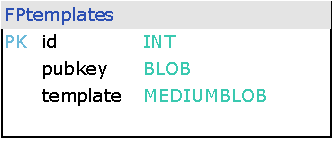
\includegraphics[width=\textwidth/2]{obrazky-figures/databaza.pdf}
	\caption{Schéma tabuľky v~MySQL databáze.}
	\label{pic_database}
\end{figure}

\section{Blockchain}
V~tejto sekcii bude popísaná implementácia samotného Blockchainu a spôsobu komunikácie so systémom. Blockchain využíva konsenzus protokol typu PoA, konkrétne jednu z~verzií jeho implementácie pre blockchain Ethereum s~názvom Clique. Špecifikácia blockchainu je uložená v~jeho konfiguračnom súbore s~názvom \texttt{genesis.json} \ref{genesis_code}.

\begin{figure}[hbt]
\renewcommand\figurename{Výpis kódu}
    \begin{boxedverbatim}
{
    "config": {
      	"chainId": 15,
      	"homesteadBlock": 0,
      	"eip150Block": 0,
      	"eip155Block": 0,
      	"eip158Block": 0,
     	"byzantiumBlock": 0,
     	"constantinopleBlock": 0,
      	"petersburgBlock": 0,
    	"clique": {
        "period": 1,
        "epoch": 30000
    	}
    },
    "difficulty": "1",
    "gasLimit": "800000",
    "extradata": "0x00000000 ...
    "alloc": {
    	"0x214bdF484d62F1ca16e19ec684845f059542fed8": { "balance": ...
    }
}
    \end{boxedverbatim}
    \caption{Konfiguračný súbor Blockchainu.}
	\label{genesis_code}
\end{figure}

Jednotlivými, pre systém dôležitými položkami konfiguračného súboru blockchainu sú:

\begin{itemize}
  \item{\texttt{chainId}, ktorý slúži pre odlíšenie siete od iných súkromných sietí. Rôzne siete, produkčné, testovacie a aj vývojové majú každá svoje unikátne \texttt{chainId}, napríklad 1 pre Ethereum \texttt{mainnnet}, 3 pre testovaciu sieť \texttt{ropsten}, 4 pre testovaciu sieť \texttt{Ropsten} atď. Pre našu sieť bolo zvolené číslo 15.}
  \item{\texttt{clique}, čo značí použitie rovnomenného konsenzus protokolu. V~rámci tohoto protokolu je nastavený parameter \texttt{period}, ktorý udáva dĺžku vytvárania bloku v~sekundách a v~prípade implementovaného systému je nastavený na hodnotu 1. Parameter \texttt{epoch} reprezentuje dĺžku epochy udávanú v~počte blokov. V~našom prípade je nastavený na hodnotu 300}
  \item{\texttt{extradata} obsahuje prvotné adresy validátorských uzlov v~sieti. Je formát sa skladá z~32 nulových bajtov, ktoré nasledujú všetky adresy validátorských uzlov za sebou. Za adresami nasleduje ďalších 65 bajtov s~hodnotou nula.}
  \item{\texttt{alloc} obsahuje hodnoty adries, ktoré majú byť predfinancované určitým množstvom meny, ktorú využíva daná sieť. Vzhľadom na povahu protokolu \texttt{clique} bude predfinancované množstvo tvoriť 100\% meny v~obehu siete. Z~tohoto dôvodu je potrebné dbať na zvolenie adekvátneho množstva pre splnenie účelu danej siete.}
\end{itemize}

\subsection{Stanice}
Inštancie jednotlivých staníc, ako validátorských tak aj klientskych, sú nakonfigurované na spomínanom nástroji Geth, bežiacom na operačnom systéme Windows 10.

Pre synchronizáciu a zaručenie správnej komunikácie medzi jednotlivými stanicami oboch typov je použitý \texttt{bootnode}. Ide o~špeciálny typ stanice pomocou ktorej sa stanica vie pripojiť a synchronizovať so zvyšnými stanicami v~sieti. Ostatné stanice sa na ňu vedia pripojiť pomocou jedinečného identifikátoru danej stanice zvaného \texttt{enode} a špeciálneho kľúča \texttt{nodekey}. 

Konfigurácia pre nástroj Geth, pre jednotlivé staníc je vždy uložená v~samostatnom súbore a obsahuje hodnoty jednotlivých parametrov:
\begin{itemize}
  \item{\texttt{syncmode} nastavený na \texttt{full} -- stanice vždy držia kompletnú kópiu siete}
  \item{\texttt{networkid} -- identifikátor siete do ktorej sa stanica chce pripojiť, čiže 15}
  \item{parameter \texttt{gasprice} nastavený na 1 značí validátorským staniciam aby prijímali transakcie s~minimálnou hodnotou poskytnutej meny, čo slúži na spomalenie jej obehu}
  \item{nastavenie lokálnych súborov stanice}
  \item{nastavenie použitej stanice \texttt{bootnode}}
  \item{nastavenie vypnutia komunikácie vrámci \texttt{IPC}}
  \item{konfiguráciu pripojenia pomocou \texttt{http}}
  \item{rozhrania dostupné pomocou pripojenia cez \texttt{http}}
  \item{konfigurácia ip adresy a portu stanice}
\end{itemize}

\paragraph{Pripojenie systému ku klientskej stanici a interakcia s~blockchainom}
Ako už bolo spomínané, systém sa ku stanici pripojí pomocou protokolu \texttt{http}. Túto funkcionalitu poskytuje knižnica \texttt{Web3}, slúžiaca pre interakciu s~blockchainom Ethereum. Toto komunikačné rozhranie je tvorené dvoma funkciami.

Prvou z~nich je \texttt{blockchainPull} a slúži na čítanie dát, respektíve kryptografického odtlačku, z~blockchainu. Má jeden parameter \texttt{key}, ktorý je typu \texttt{RSA.RsaKey}, reprezentujúci užívateľa, ktorému patrí hľadaný kryptografický odtlačok. Funkcia po pripojení ku stanici vytvorí inštanciu kontraktu, reprezentovaného premennou \texttt{myContract}, ktorý následne s~predaním parametra \texttt{key} aj vykoná. Návratovou hodnotou funkcie je návratová hodnota získaná vykonaním kontraktu. Táto funkcia dáta z~blockchainu iba číta, takže na jej vykonanie efektívne nie je potrebný žiadny obnos meny.

Druhou z~funkcií je \texttt{blockchainPush}, ktorá slúži na uloženie dát do blockchainu. Prijíma jeden extra parameter oproti predošlej. Extra parameter \texttt{data}, ktorý je typu \texttt{bytes}, reprezentuje kryptografický odtlačok určený na uloženie do blockchainu. Funkcia obdobne vytvorí inštanciu kontraktu, ktorý ale následne vykoná ako transakciu. Následne funkcia čaká na potvrdenie o~spracovaní transakcie. Funkcia zapisuje dáta do blockchainu čo znamená, že spotrebúva určitý obnos meny, ktorá je pre jej potreby pripravená na účte sprístupnenom na klientskej stanici.

Všetky hodnoty parametrov (adresu a port stanice, adresu predfinancovaného účtu a \texttt{ABI} kontraktu) funkcie získajú z~konfiguračného súboru systému. Obe funkcie taktiež využívajú vrstvu kompatibility určenú pre pripojenie ku sieťam, ktoré využívajú konsenzus protokol PoA. Táto vrstva je nutná kvôli neštandardnej dĺžke parametru \texttt{extradata} v~konfiguračnom súbore blockchainu.

\subsection{Smart kontrakt}
Smart kontrakt je napísaný v~programovacom jazyku Solidity a nachádza sa uložený v~súbore \texttt{storage.sol}. Obsahuje dve funkcie, jeden event a zoznam štruktúr.

Dáta jedného užívateľa sú reprezentované štruktúrou \texttt{User}, ktorá obsahuje dve položky, \texttt{pubkey} a \texttt{templatehash}. Prvá z~nich je typu \texttt{bytes}, ktorý umožňuje uloženie variabilného počtu bajtov a reprezentuje identifikátor, respektíve súkromný kľúč užívateľa. Druhá je typu \texttt{bytes32} a umožňuje uloženie dát o~veľkosti 32 bajtov. Táto premenná slúži na uloženie kryptografického odtlačku šablóny užívateľa. Vrámci kontraktu sú všetky užívateľské dáta uložené v~zozname štruktúr typu \texttt{User}, nazvanom \texttt{users}.

Manipuláciu s~dátami zabezpečujú dve funkcie. Prvá z~nich, \texttt{store}, slúži na zápis dát do blockchainu. Prijíma dva parametre, \texttt{key} a \texttt{hash}, oba v~bajtovej podobe. Po zapísaní dát do blockchainu funkcia vyvolá event. Ten má v~blockchaine Ethereum viacero využití no v~tomto prípade bol použitý pre účely auditovateľnosti. Event slúži na zapísanie správy s~určitými parametrami do denníku siete. Event má v~implementovanom kontrakte názov \texttt{Enroll}, a ako parametre prijíma položky štruktúry \texttt{User}. Správy sú do denníku siete zapísané permanentne, čo znamená, že pomocou nich je možné spoľahlivo určiť vykonané zmeny dát.

Druhá funkcia slúži na čítanie dát a prijíma jeden parameter \texttt{key}, taktiež typu \texttt{bytes}. Funkcia postupne prechádza všetkými položkami zoznamu \texttt{users} a hľadá zhodu v~položke \texttt{pubKey} a vstupnom parametri. Ak ju nájde, vráti hodnotu premennej \texttt{templateHash} daného záznamu. Naopak, v~prípade neúspešného vyhľadávania, vráti hodnotu 0.

\paragraph{Nasadenie}
Pre tento účel bola v~systéme implementovaná funkcia \texttt{deployContract}. Po pripojení ku klientskej stanici funkcia prečíta zdrojový kód smart kontraktu zo súboru \texttt{storage.sol}, ktorý následne preloží pomocou knižnice \texttt{solcx}. Po preložení sú \texttt{ABI} a preložený kontrakt uložené do konfiguračného súboru systému. \texttt{ABI} poskytuje informácie o~rozhraní daného kontraktu a je spolu s~jeho adresou nevyhnutné pre ďalšiu interakciu. Nakoľko nasadenie smart kontraktu do blockchainu je úkon, ktorý spotrebúva menu, je na stanici pripravený predfinancovaný účet. Funkcia následne kontrakt nasadí do blockchainu a počká na potvrdenie o~úspešnosti transakcie. Ako posledný krok je z~potvrdenia o~úspešnosti transakcie vybratá adresa kontraktu, ktorá je následne uložená do konfiguračného súboru systému.

\subsection{Pomocné funkcie a súbory}
Jedná sa o~funkcie, ktoré slúžia na prípravu systému pred prvotným spustením a jeho demonštráciu.

\paragraph{\texttt{badexit}} je funkcia slúžiaca na ukončenie programu pri narazení na chybu. Program je ukončený s~návratovým kódom 1.

\paragraph{\texttt{loadKey}} slúži na načítanie kľúča zo súboru, ktorého názov je predaný pomocou parametra \texttt{filename}. Funkcia vracia objekt typu \texttt{Crypto.RSA.RsaKey}

\paragraph{\texttt{generateKeys}}  Systém poskytuje užívateľom možnosť vytvoriť pre nich nový súkromný a verejný kľúč. Požadovaná veľkosť v~bitoch je určená parametrom \texttt{size}. Funkcia vygenerované kľúče uloží vo formáte PEM do dvoch samostatných súborov \texttt{key\_pub.pem} a \texttt{key\_sec.pem}

\paragraph{\texttt{deleteBlockchainData}} je funkcia slúžiaca na vymazanie lokálnych kópií dát blockchainu. Funkcia prechádza adresáre jednotlivých lokálnych staníc a vymazáva z~nich adresár \texttt{geth} spolu s~jeho obsahom.

\paragraph{\texttt{blockchainStart}} spúšťa powershell skript \texttt{blockchain\_start.ps1}. Samotný skript inicializuje a spúšťa päť inštancií lokálnych staníc. Jedna z~nich je \texttt{bootnode}, tri sú validátorské a jedna je klientska.

\paragraph{\texttt{blockchainStart}} slúži čisto na demonštračné účely. Prijíma tri parametre, ktorými sú  \texttt{victimPubKey}, \texttt{attackerPubKey} a \texttt{attackerTemplate}. Funkcia skompromituje databázový systém nahradením šablóny obete šablónou útočníka, ktorá je taktiež zašifrovaná jeho verejným kľúčom.

\section{Beh programu}

Beh implementovaného programu môžeme rozdeliť do štyroch vetiev podľa toho, čo chceme aby vykonal. Ovládanie programu sa vykonáva pomocou príkazu a argumentov. Po ich spracovaní sa program koná následovne.

\paragraph{Príprava}
V~tohoto príkazu na prípravu program vykoná prípravu podľa zadaných parametrov, ktoré zahŕňajú:
\begin{itemize}
  \item{generovanie nového kľúčového páru -- v~prípade ak ním užívateľ ešte nedisponuje}
  \item{inicializácia databázového systému -- program vytvorí na databázovom serveri novú tabuľku podľa špecifikácie \ref{pic_database}, prípadne ju prv zmaže ak existuje}
  \item{inicializácia blockchainu -- program zmaže lokálne dáta blockchainu a nanovo, pomocou súboru \texttt{genesis.json}, inicializuje a spustí päť lokálnych staníc. Z~nich je jedna \texttt{bootnode}, tri validátorské a jedna klientska}
  \item{inštalácia prekladača pre programovací jazyk Solidity}
  \item{nasadenie kontraktu do blockchainu}
\end{itemize}

\paragraph{Zápis užívateľa}
Prebieha troch krokoch. Užívateľ na vstupe poskytne svoju biometrickú šablónu a verejný kľúč. V~provom kroku je šablóna zašifrovaná hybridnou šifrou s~použitím verejného kľúča. V~druhom kroku je táto zašifrovaná šablóna spolu s~verejným kľúčom uložená do databázy. Na záver je zo zašifrovanej šablóny vypočítaný kryptografický odtlačok, ktorý je následne, spolu s~verejným kľúčom, uložený do blockchainu.

\paragraph{Autentifikácia užívateľa}
Pre úspešnú autentifikáciu potrebuje užívateľ správny verejný a hlavne súkromný kľúč a taktiež zhodnú biometrickú šablónu. Všetky tieto položky sú programu predané na vstupe.
V~prvej fáze autentifikácie sa v~databázovom systéme vyhľadá zašifrovaná šablóna, pričom následne prebehne overenie jej integrity. V~blockchaine sa vyhľadá kontrolný kryptografický odtlačok, ktorý je porovnaný s~odtlačkom vytvoreným zo stiahnutej šablóny. V~prípade, ak je hľadanie podľa verejného kľúča v~blockchaine alebo v~databázovom systéme neúspešné, program skončí s~oznámením o~chybe a návratovou hodnotou 1. Ak sú odtlačky totožné, je úspešne overená integrita stiahnutej šablóny a systém ďalej pokračuje jej dešifrovaním. V~prípade, že používateľ, ktorý sa pokúša o~autentifikáciu poskytne správny súkromný kľúč, je šablóna úspešne dešifrovaná a porovnaná so vstupnou. Výsledok autentifikácie je používateľovi ukázaný prostredníctvom konzolového výpisu.

\paragraph{Demonštrácia kompromitácie}
Systém obsahuje možnosť demonštratívne skompromitovať databázový systém. Na vstupe je zadaný užívateľ, ktorý má byť skompromitovaný, vo forme jeho verejného kľúča spolu s~verejným kľúčom a biometrickou šablónou útočníka. Databázový záznam užívateľa je upravený nahradením jeho autentickej šablóny za útočníkovu, ktorá je zároveň zašifrovaná jeho kľúčom. Útočník sa následne môže pokúsiť autentifikovať ako užívateľ za použitia svojej biometrickej šablóny a súkromného kľúča.

\chapter{Testovanie a vyhodnotenie}
Táto kapitola obsahuje popis vykonaných testov, ktorých účelom bolo zhodnotenie funkčnosti, odhalenie chýb a zistenie či implementovaný systém spĺňa svoj účel.
Pre potreby testovania boli vytvorené dva kľúčové páry a dva súbory reprezentujúce biometrické šablóny.

\section{Testovanie funkčnosti}
V~rámci testovania systému bude vykonaná príprava pre prvým použitím užívateľmi, čo znamená vytvorenie databáze, spustenie blockchainu a nasadenie smart kontraktu. Na otestovanie základnej funkcionality a chovania systému budú vykonané tri testy a pre testovanie odolnosti voči útoku na databázový systém bude vykonaný jeden test. Cieľom testov vykonaných v~tejto sekcii je otestovať základnú funkcionalitu systému a jeho chovanie v~prípade pokusu o~útok.

\subsection{Príprava}
Spočíva v~dvoch spusteniach \ref{terminal0} systému, pri prvom je inicializovaný databázový systém a spustený blockchain a pri druhom je do blockchainu nasadený kontrakt.
\begin{figure}[hbt]
\renewcommand\figurename{Výpis kódu}
\begin{Verbatim}[frame=single]
python3 .\system.py setup --database --blockchain
python3 .\system.py setup --contract
\end{Verbatim}
    \caption{Príkazy pre test prípravy systému.}
	\label{terminal0}
\end{figure}

Prvé spustenie prebehlo úspešne, o~čom nás aj systém výpisom informoval. Kontrolou pomocou nástroja \texttt{phpMyAdmin} bežiaceho priamo na databázovom serveri bolo potvrdené korektné vytvorenie tabuľky. Z~výstupu nástroja Geth v~termináli, v~ktorom bol systém spustený, môžeme vidieť úspešnú inicializáciu jednotlivých lokálnych staníc. Taktiež na novootvorených termináloch je možné vidieť prácu blockchainu t.j. stanice spolu komunikujú, vytvárajú, validujú a distribuujú si medzi sebou bloky.
Druhé spustenie taktiež prebehlo podľa očakávania, kontrakt bol úspešne nasadený do blockchainu. Toto vieme potvrdiť jednak podľa výpisu z~terminálu lokálnej klientskej stanice, ale aj nahliadnutím do konfiguračného súboru systému, kde môžeme vidieť, že systém úspešne zapísal adresu kontraktu získanú z~potvrdenia o~jeho úspešnom nasadení.

\subsection{Zápis užívateľa}
V~tomto teste bude systém opäť spustený dva krát \ref{terminal1}, pre zápis dvoch rôznych užívateľov. Program bude spustený s~prepínačom \texttt{verbose}, ktorý aktivuje rozšírený výpis. Očakávaným výstupom je úspešný zápis do systému.

\begin{figure}[hbt]
\renewcommand\figurename{Výpis kódu}
\begin{Verbatim}[frame=single]
python3 .\system.py enroll --key .\keys\key_pub1.pem --template .\template
s\template1 --verbose
python3 .\system.py enroll --key .\keys\key_pub2.pem --template .\template
s\template2 --verbose
\end{Verbatim}
    \caption{Príkazy test zápisu užívateľa.}
	\label{terminal1}
\end{figure}

Obe spustenia prebehli podľa systému úspešne. Overenie korektnosti dát nahraných do databázy bolo vykonané za pomoci nástroja \texttt{phpMyAdmin} ich manuálnym stiahnutím a porovnaním pomocou nástroja \texttt{diff}. Zároveň podľa výpisu z~terminálu klientskej stanice vidíme že zápis kryptografického odtlačku ňou bol spracovaný.

\subsection{Autentifikácia užívateľa}
Po úspešnom zápise je nasledujúcim testom autentifikácia  užívateľov. Systém bude opäť spustený dva krát \ref{terminal2}, pre oboch zapísaných užívateľov, za použitia korektných autentifikačných prostriedkov. Očakávaným výstup je v~oboch prípadoch úspešná kontrola integrity šablóny z~databázy a následne aj úspešná autentifikácia.

\begin{figure}[hbt]
\renewcommand\figurename{Výpis kódu}
\begin{Verbatim}[frame=single]
python3 .\system.py authenticate --keys .\keys\key_pub1.pem .\keys\key_sec
1.pem --template .\templates\template1 --verbose
python3 .\system.py authenticate --keys .\keys\key_pub2.pem .\keys\key_sec
2.pem --template .\templates\template2 --verbose
\end{Verbatim}
    \caption{Príkazy pre test úspešnej autentifikácie užívateľa.}
	\label{terminal2}
\end{figure}

Na výstupe \ref{terminal3} oboch spustení programu môžme vidieť, že overenie integrity aj autentifikácia užívateľa prebehli úspešne. Zároveň porovnaním jednotlivých položiek rozšíreného výstupu programu je opäť evidentná ich zhoda a aj celkový úspech testu.

\begin{figure}[hbt]
\renewcommand\figurename{Výpis kódu}
\begin{Verbatim}[frame=single]
RUNNING AUTHENTICATION ...
        Retrieving template from database ... DONE
        Retrieving hash from blockchain ... DONE
        Checking data integrity ... VALID
        Decrypting template ... DONE
        Comparing templates ... MATCH
AUTHENTICATION DONE
\end{Verbatim}
    \caption{Výstup úspešnej autentifikácie užívateľa.}
	\label{terminal3}
\end{figure}

\subsection{Odmietnutie prístupu}
Tento test slúži na preukázanie schopnosti systému odmietnuť prístup užívateľa v~prípade, že nedisponuje korektnými autentifikačnými prostriedkami. Systém bude celkovo spustený dva krát \ref{terminal4}, prvý krát s~nesprávnym súkromným kľúčom a druhý krát s~nezhodujúcou sa šablónou. Očakávaným výstupom je úspešné overenie integrity no neúspešná autentifikácia.

\begin{figure}[hbt]
\renewcommand\figurename{Výpis kódu}
\begin{Verbatim}[frame=single]
python3 .\system.py authenticate --keys .\keys\key_pub1.pem .\keys\key_sec
2.pem --template .\templates\template1 --verbose
python3 .\system.py authenticate --keys .\keys\key_pub1.pem .\keys\key_sec
1.pem --template .\templates\template2 --verbose
\end{Verbatim}
    \caption{Príkazy pre test neúspešnej autentifikácie užívateľa.}
	\label{terminal4}
\end{figure}

Výstup \ref{terminal5} prvého spustenia podľa očakávania ukazuje chybu pri pokuse systému o~dešifrovanie šablóny z~databázy, ktorá znamená, že užívateľ nedisponuje korektným súkromným kľúčom.
\begin{figure}[hbt]
\renewcommand\figurename{Výpis kódu}
\begin{Verbatim}[frame=single]
RUNNING AUTHENTICATION ...
        Retrieving template from database ... DONE
        Retrieving hash from blockchain ... DONE
        Checking data integrity ... VALID
        Decrypting template ... Data decryption(RSA) failed
ERROR
\end{Verbatim}
    \caption{Výstup neúspešnej autentifikácie užívateľa (nesprávny súkromný kľúč).}
	\label{terminal5}
\end{figure}

Výstup \ref{terminal6} druhého spustenia ukazuje, že overenie integrity a dešifrovanie prebehlo úspešne, no systém nenašiel zhodu medzi referenčnou a vstupnou šablónou. Rozdiel medzi vstupnou šablónou a šablónou z~databázy je opäť možné vidieť na rozšírenom výstupe. Test tým pádom skončil úspechom.
\begin{figure}[hbt]
\renewcommand\figurename{Výpis kódu}
\begin{Verbatim}[frame=single]
RUNNING AUTHENTICATION ...
        Retrieving template from database ... DONE
        Retrieving hash from blockchain ... DONE
        Checking data integrity ... VALID
        Decrypting template ... DONE
        Comparing templates ... NO MATCH
AUTHENTICATION DONE
\end{Verbatim}
    \caption{Výstup neúspešnej autentifikácie užívateľa (nesprávna vstupná šablóna).}
	\label{terminal6}
\end{figure}

\subsection{Detekcia kompromitácie databázy}
Posledný z~testov \ref{terminal7} slúži na potvrdenie schopnosti systému detegovať neoprávnené zmeny dát v~databáze, konkrétne pokus o~vydávanie sa za legitímneho užívateľa zámenou zašifrovanej šablóny za skompromitovanú. Prvé spustenie slúži na demonštračnú kompromitáciu databázy a druhé reprezentuje pokus útočníka o~autentifikáciu. Očakávaným výstupom je úspešná detekcia porušenia integrity databázy.

\begin{figure}[hbt]
\renewcommand\figurename{Výpis kódu}
\begin{Verbatim}[frame=single]
python3 .\system.py compromise --victim .\keys\key_pub1.pem --attacker .\k
eys\key_pub2.pem --template .\templates\template2 --verbose
python3 .\system.py authenticate --keys .\keys\key_pub1.pem .\keys\key_sec
2.pem --template .\templates\template2 --verbose
\end{Verbatim}
    \caption{Príkazy pre kompromitáciu a následný pokus o~autentifikáciu.}
	\label{terminal7}
\end{figure}

Pri pohľade na výstup \ref{terminal8} druhého spustenia je vidieť, že systém úspešne zachytil podvrhnutú šablónu z~databázy. Taktiež je z~rozšíreného výstupu viditeľný rozdiel medzi kryptografickým odtlačkom dát z~databázy a tým, ktorý bol získaný z~blockchainu. Test odhalil porušenie integrity databázy a skončil úspechom.
\begin{figure}[hbt]
\renewcommand\figurename{Výpis kódu}
\begin{Verbatim}[frame=single]
RUNNING AUTHENTICATION ...
        Retrieving template from database ... DONE
        Retrieving hash from blockchain ... DONE
        Checking data integrity ... INVALID
        Decrypting template ... DONE
        Comparing templates ... MATCH
AUTHENTICATION DONE
\end{Verbatim}
    \caption{Výstup neúspešnej autentifikácie útočníka.}
	\label{terminal8}
\end{figure}


\section{Testovanie výkonnosti}
Po otestovaní základnej funkcionality aplikácie nasledovalo testovanie rýchlosti systému. Testované boli systémové úkony, pri ktorých je predpoklad, že budú vykonávané najčastejšie, čiže zápis nového užívateľa a jeho autentifikácia. Každý z~týchto úkonov bol testovaný pri rôznych počtoch lokálnych staníc, pričom pri každom bol program spustený celkom deväť krát. Trvanie behu programu bolo merané pomocou nástroja \texttt{Measure-Command} na operačnom systéme Windows 10 bežiacom na procesore Intel(R) Core(TM) i7-7700HQ.

Výsledky testov zápisu užívateľa môžeme vidieť v~tabuľke \ref{perftest}, ktorá obsahuje priemerné hodnoty trvania a ich rozptyl. Môžeme z~nich vidieť, že samotné trvanie zápisu v~tomto prípade nezávisí od počtu validároských uzlov v~sieti. Rozdiel medzi najrýchlejšou a najpomalšou dobou bol približne 12\%. V~prípade doby trvania autentifikácie užívateľa bola priemerná hodnota 1,395266488 sekundy. Tá sa s~rôznym počtom validátorských uzlov v~sieti nebude líšiť, nakoľko proces autentifikácie dáta z~blockchainu iba číta a tým pádom je táto operácia vykonávaná iba klientskou stanicou, nie celým blockchainom.

Pri interpretácii výsledkov treba brať ohľad na variabilitu spôsobenú inými aktuálne spustenými aplikáciami na operačnom systéme.

\begin{table}[h]
\resizebox{\textwidth}{!}{%
\begin{tabular}{|c|c|c|}
\hline
Počet validátorských uzlov & Priemerné trvanie zápisu do systému (s) & Rozptyl trvania zápisu do systému (s)\\ \hline
3  & 2,943587 & 0,031703 \\
4  & 2,944505 & 0,172852 \\
5  & 3,155935 & 0,14433  \\
6  & 3,041142 & 0,037279 \\
7  & 3,354695 & 0,12212  \\
8  & 3,128044 & 0,357989 \\
9  & 3,202814 & 0,41072  \\
10 & 3,101774 & 0,096156 \\ \hline
\end{tabular}%
}
\caption{Výsledky merania výkonnosti}
\label{perftest}
\end{table}


\section{Vyhodnotenie}
Navrhnutý systém obstál v~pripravených testoch funkčnosti, ktoré zastrešovali základnú cielenú funkcionalitu. Cieľom taktiež bolo aby navrhnutý systém využíval decentralizovaný prístup k~autentifikácii s~dôrazom integritu úložiska biometrických šablón. Tento cieľ systém spĺňa svojím mechanizmom pre kontrolu integrity databázového systému, ktorý využíva blockchain. Decentralizovaná povaha systému je ďalej podporovaná zverením kľúča zabezpečenia biometrických údajov do rúk užívateľa.

\paragraph{}
Žiadny systém nemožno označiť za bezpodmienečne bezpečný Tým je len do vtedy kým nie je preukázaný opak. V~nasledujúcej časti budú diskutované bezpečnostné nedostatky navrhnutého systému.
\paragraph{}

Zverenie šifrovacích kľúčov do rúk užívateľa mu síce dáva väčšiu kontrolu nad zabezpečením svojich dát, no zároveň sa na neho kladie aj zodpovednosť za ich korektné uloženie a ochranu pred kompromitovaním. Pri ich skompromitovaní alebo nebodaj strate bude nenávratne kompromitovaná aj identita užívateľa, čo vyplýva aj z~povahy technológie.
\paragraph{}

Jednou zo zraniteľností systému je možnosť napadnutia komunikačného kanálu medzi zariadením, na ktorom beží klientska aplikácia a klientskou stanicou, ktorá slúži na interakciu s~blockchainom. V~tomto prípade by mohlo dôjsť ku zámene kryptografického odtlačku vo fáze zápisu alebo autentifikácie, čím by v~konečnom dôsledku mohol byť skompromitovaný celý systém. Možným riešením by bola užšia integrácia klientskej aplikácie a stanice, prípadne ich úplné spojenie.
\paragraph{}

Mechanizmus kontroly integrity databázového systému závisí na integrite blockchainu. Tá je v~prípade použitého protokolu garantovaná ak je podiel byzantských uzlov v~sieti pod polovicou počtu všetkých uzlov. V~prípade, že by sa táto podmienka porušila, mohlo by dôjsť ku nelegitímnej manipulácii dát uložených v~blockchaine, čím by bol systém skompromitovaný.
\paragraph{}

Použitie databázového systému vnieslo do navrhovaného systému centralizovaný prvok. Tým sa systém stal náchylným voči cielenému útoku na jediný bod, a to databázový systém. Aj keď uložené dáta sú zabezpečené, takýto útok by znamenal uvedenie systému mimo prevádzky. Táto zraniteľnosť je riešiteľná použitím distribuovaného dátového úložiska. V~rámci tohoto úložiska by mali dáta byť uložené s~určitou mierou redundancie a rozmiestnené na servery umiestnené na rôznych lokalitách a sieťach.

Celkovo by sa dôveryhodnosť systému dala zvýšiť jeho presunom, prípadne určitej jeho časti, z~klientskej aplikácie do blockchainu a tým z~neho spraviť plne decentralizovanú aplikáciu.

\chapter{Záver}
V~rámci tejto práce bol navrhnutý a implementovaný systém pre realizáciu biometrickej autentifikácie, ktorý zároveň disponuje mechanizmom pre detekciu porušenia integrity úložiska biometrických šablón. V~priebehu práce bolo nutné naštudovať biometrické autentifikačné systémy, ako centralizované tak aj decentralizované, a technológiu blockchain. Cieľom práce bolo zakomponovať do výsledného systému technológiu blockchain. Navrhovaný systém mal zároveň za cieľ byť decentralizovaného charakteru.

Implementovaný systém má formu aplikácie spolupracujúcej s~databázovým systémom a blockchainom, ktorá vykonáva zápis a autentifikáciu užívateľov. Cielená funkcionalita detekcie porušenia integrity úložiska bola úspešne navrhnutá a implementovaná za pomoci blockchainu bežiaceho v~privátnom nastavení. Decentralizovaný charakter aplikácie bol naplnený využitím blockchainu pre kontrolu integrity a poskytnutím kontroly nad zabezpečením dát samotnému užívateľovi.

Testovanie systému dosiahlo vyhovujúce výsledky. Systém bol schopný splniť základnú funkcionalitu v~kontrolovanom prostredí a predpokladá sa aj dobrá úroveň škálovateľnosti. Testovanie neodhalilo chyby funkcionality. Systém obsahoval určité bezpečnostné medzery, z~ktorých boli niektoré identifikované a bolo navrhnuté aj ich riešenie.

Možným ďalším smerovaním práce by bolo vyriešenie nedostatkov vzhľadom na bezpečnosť a úplná eliminácia centralizovaných prvkov systému a to napríklad využitím distribuovaného úložiska alebo úplným presunom funkcionality klientskej aplikácie do blockchainu.

